\documentclass[11pt,a4paper,oneside]{report}

% ==============================================================================
% PACKAGES & CONFIGURATION
% ==============================================================================
\usepackage[utf8]{inputenc}
\usepackage[T1]{fontenc}
\usepackage{lmodern}
\usepackage[margin=0.9in,top=0.9in,bottom=0.9in]{geometry}
\usepackage{setspace}
\setstretch{1.15} % Standard readable academic line spacing

\usepackage{graphicx}
\usepackage{xcolor}
\usepackage{booktabs}
\usepackage{tabularx}
\usepackage{longtable}
\usepackage{array}
\usepackage{amsmath,amssymb}
\usepackage{sectsty}
\usepackage{fancyhdr}
\usepackage{microtype}
\usepackage{listings}
\usepackage{tcolorbox}
\usepackage{caption}
\usepackage{subcaption}
\usepackage{float}
\usepackage{hyperref}

% Color definitions
\definecolor{primaryblue}{RGB}{14, 116, 144}   % Medical Cyan/Teal
\definecolor{darknavy}{RGB}{15, 23, 42}       % Dark Slate
\definecolor{accentgreen}{RGB}{16, 185, 129}   % Health Green
\definecolor{codegray}{RGB}{245, 247, 250}
\definecolor{bordergray}{RGB}{226, 232, 240}
\definecolor{codeblue}{RGB}{2, 132, 199}

% Hyperref setup
\hypersetup{
    colorlinks=true,
    linkcolor=primaryblue,
    citecolor=primaryblue,
    urlcolor=codeblue,
    pdfauthor={Riduanul Abedin Shihab},
    pdftitle={Technical Internship and Project Report: National Hospital Chattogram},
    pdfsubject={Flutter and Supabase Digital Healthcare Ecosystem}
}

% Code listing style
\lstdefinestyle{codeStyle}{
    backgroundcolor=\color{codegray},
    basicstyle=\ttfamily\footnotesize,
    breakatwhitespace=false,
    breaklines=true,
    captionpos=b,
    keepspaces=true,
    numbers=left,
    numbersep=7pt,
    numberstyle=\tiny\color{gray},
    showspaces=false,
    showstringspaces=false,
    showtabs=false,
    tabsize=2,
    frame=single,
    rulecolor=\color{bordergray},
    keywordstyle=\color{primaryblue}\bfseries,
    commentstyle=\color{gray}\itshape,
    stringstyle=\color{accentgreen}
}
\lstset{style=codeStyle}

% Header and Footer setup
\pagestyle{fancy}
\fancyhf{}
\fancyhead[L]{\parbox[b]{0.44\textwidth}{\raggedright\footnotesize\textsf{\color{darknavy}National Hospital Chattogram}}}
\fancyhead[R]{\parbox[b]{0.54\textwidth}{\raggedleft\footnotesize\textsf{\color{gray}\nouppercase{\leftmark}}}}
\fancyfoot[C]{\thepage}
\renewcommand{\headrulewidth}{0.4pt}
\setlength{\headheight}{24pt}
\addtolength{\topmargin}{-8pt}

% Section and Chapter Heading Styling
\chapterfont{\color{darknavy}\sffamily\huge}
\sectionfont{\color{darknavy}\sffamily\Large}
\subsectionfont{\color{primaryblue}\sffamily\large}

% ==============================================================================
% DOCUMENT BEGIN
% ==============================================================================
\begin{document}

% ------------------------------------------------------------------------------
% TITLE PAGE
% ------------------------------------------------------------------------------
\begin{titlepage}
    \centering
    \vspace*{0.2cm}
    
    % Premier University Official Logo
    
\includegraphics[width=2.8cm]{assets/images/premier_university_logo.png}\\[0.35cm]
    
    {\Huge \textbf{\textsf{\color{darknavy}PREMIER UNIVERSITY, CHITTAGONG}}}\\[0.2cm]
    {\Large \textsf{\color{gray}Department of Computer Science \& Engineering}}\\[0.6cm]
    
    \rule{\textwidth}{1.6pt}\\[0.35cm]
    {\LARGE \textbf{\textsf{\color{darknavy}COMPREHENSIVE INTERNSHIP REPORT}}}\\[0.25cm]
    {\large \textbf{\textsf{\color{primaryblue}NATIONAL HOSPITAL CHATTOGRAM: DIGITAL HEALTHCARE PLATFORM \& MANAGEMENT ECOSYSTEM}}}\\[0.15cm]
    {\normalsize \textsf{Patient Mobile Application \& Standalone Web Admin Control Panel}}\\[0.35cm]
    \rule{\textwidth}{1.6pt}\\[0.5cm]
    
    \begin{tcolorbox}[colback=codegray,colframe=primaryblue!50,arc=2mm,width=0.96\textwidth]
        \centering\large
        \textbf{COURSE CODE:} CSE 4001 \quad\textbar\quad 
        \textbf{COURSE TITLE:} Internship \quad\textbar\quad 
        \textbf{SESSION:} Spring-2026
    \end{tcolorbox}
    
    \vspace{1.2cm}
    
    \begin{minipage}[t]{0.48\textwidth}
        \textbf{\large Prepared By:}\\[0.25cm]
        {\large \textbf{Riduanul Abedin Shihab}}\\[0.15cm]
        \textbf{Student ID:} 0222220005101164\\[0.12cm]
        Program: B.Sc. in CSE\\[0.12cm]
        Department of Computer Science \& Engineering\\[0.12cm]
        Premier University, Chittagong
    \end{minipage}
    \hfill
    \begin{minipage}[t]{0.48\textwidth}
        \begin{flushright}
            \textbf{\large Supervised By:}\\[0.25cm]
            {\large \textbf{Mr. Tanvir Hassan Ananta}}\\[0.15cm]
            Lecturer\\[0.12cm]
            Department of Computer Science \& Engineering\\[0.12cm]
            Premier University, Chittagong
        \end{flushright}
    \end{minipage}
    
    \vfill
    
    {\large \textbf{Submission Date: 2 November 2026}}
\end{titlepage}

% ------------------------------------------------------------------------------
% PRELIMINARY PAGES
% ------------------------------------------------------------------------------
\pagenumbering{roman}

\chapter*{Certificate of Approval}
\addcontentsline{toc}{chapter}{Certificate of Approval}
This is to certify that the internship report entitled \textbf{``National Hospital Chattogram: Digital Healthcare Platform \& Management Ecosystem''} submitted for \textbf{COURSE CODE: CSE 4001} (\textbf{COURSE TITLE: Internship}, \textbf{SESSION: Spring-2026}) by \textbf{Riduanul Abedin Shihab} (Student ID: \texttt{0222220005101164}) in partial fulfillment of the requirements for the degree of Bachelor of Science in Computer Science and Engineering from Premier University, Chittagong, has been examined and approved.

The 15-day internship was successfully completed under our joint academic and industrial supervision.

\vspace{2.5cm}
\noindent
\begin{minipage}{0.52\textwidth}
    \rule{6.8cm}{0.6pt}\\
    \textbf{Mr. Tanvir Hassan Ananta}\\
    Faculty Internship Supervisor \& Lecturer\\
    Department of Computer Science \& Engineering\\
    Premier University, Chittagong
\end{minipage}
\hfill
\begin{minipage}{0.45\textwidth}
    \begin{flushright}
        \rule{6.2cm}{0.6pt}\\
        \textbf{Imtiaz Riad}\\
        Company Mentor \& Technical Lead\\
        Authentic Four Technology\\
        Software Technology Park, Agrabad, Chattogram
    \end{flushright}
\end{minipage}

\clearpage

\chapter*{Declaration}
\addcontentsline{toc}{chapter}{Declaration}
I hereby declare that this internship and technical project report entitled \textbf{``National Hospital Chattogram: Digital Healthcare Platform \& Management Ecosystem''} submitted for \textbf{COURSE CODE: CSE 4001} (\textbf{COURSE TITLE: Internship}, \textbf{SESSION: Spring-2026}) is an authentic record of original work carried out by me during my 15-day internship under the academic supervision and guidance of my Faculty Internship Supervisor, \textbf{Mr. Tanvir Hassan Ananta}, Lecturer, Department of Computer Science \& Engineering, Premier University, Chittagong, alongside the industrial mentorship of \textbf{Imtiaz Riad} at Authentic Four Technology.

This work was conducted in fulfillment of the internship requirements and has not been submitted previously in substance for any degree or diploma to any other university or institute.

\vspace{1.5cm}
\noindent
\begin{minipage}{0.55\textwidth}
    \rule{6.5cm}{0.6pt}\\
    \textbf{Riduanul Abedin Shihab}\\
    Student ID: \texttt{0222220005101164}\\
    Department of Computer Science \& Engineering\\
    Premier University, Chittagong\\
    Date: 2 November 2026
\end{minipage}

\clearpage

\chapter*{Executive Abstract}
\addcontentsline{toc}{chapter}{Executive Abstract}
This report details the end-to-end design, architectural formulation, engineering execution, and deployment of the next-generation digital healthcare ecosystem for \textbf{National Hospital Chattogram}, a leading tertiary healthcare institution in Bangladesh. Healthcare operations across the region have historically suffered from paper-reliant chamber appointments, unpredictable doctor arrival schedules, telephone congestion, and manual administrative rosters prone to human error.

To resolve these systematic bottlenecks, a decoupled, multi-platform software ecosystem was architected and developed during the 15-day internship tenure starting from 1 September 2026. The ecosystem comprises:
\begin{enumerate}
    \item \textbf{Patient Mobile \& Web Portal (\texttt{/})}: A cross-platform Flutter application tailored with comprehensive Bengali localization, phone-first pre-confirmed authentication, live chamber visiting schedule tracking, Top Doctors curation, and concurrency-guaranteed digital serial booking.
    \item \textbf{Standalone Web Admin Panel (\texttt{/admin\_panel})}: An isolated Flutter Web back-office portal designed for administrative officers and reception desks to manage doctor directories, dynamically rank featured specialists, curate specialties, monitor real-time serial queues, and review immutable security audit logs.
    \item \textbf{High-Performance Persistence Layer (\texttt{Supabase / PostgreSQL 15+})}: A secured database architecture utilizing Row Level Security (RLS), custom PL/pgSQL stored procedures (RPCs), partial unique indexing to mathematically prevent double-booking, and Role-Based Access Control (RBAC).
\end{enumerate}

The report describes the 15-day internship hosted by Authentic Four Technology starting from 1 September 2026, with the final project deliverable and technical report submitted on 2 November 2026. It documents the project scope, design, implementation, technical decisions, and learning outcomes.

\clearpage
\tableofcontents
\clearpage
\listoffigures
\listoftables
\clearpage

\pagenumbering{arabic}

% ------------------------------------------------------------------------------
% CHAPTER 1: INTRODUCTION
% ------------------------------------------------------------------------------
\chapter{Introduction}

\section{Background and Purpose}
An internship connects academic learning with professional practice. This internship at Authentic Four Technology gave me the chance to apply modern software engineering and digital healthcare platform development while observing how a Bangladeshi software company designs, delivers, and supports digital products. Scalable, high-reliability software systems are increasingly vital for business operations, enterprise ERP, hospital management, and telemedicine ecosystems. This motivated my project topic: designing, engineering, and deploying a production-grade digital healthcare platform and administrative ecosystem for \textbf{National Hospital Chattogram}.

\section{Internship Objectives}
The core objectives of the internship included:
\begin{enumerate}
    \item Understand the company's business, services, structure, and technology stack.
    \item Plan and carry out an end-to-end software engineering project, from requirements gathering and relational schema modeling to frontend interface development, testing, and technical documentation.
    \item Learn professional practices such as version control, reproducible workflows, Agile delivery, and clear technical reporting.
    \item Identify healthcare operational bottlenecks and propose practical, high-performance software solutions.
    \item Develop communication, time-management, problem-solving, and teamwork skills.
\end{enumerate}

\section{Scope and Method of the Report}
The report combines three primary sources:
\begin{enumerate}
    \item Public information about Authentic Four Technology from its official website (\url{https://www.authenticfour.com}) and verified business directory listings (Tracxn and BINFO).
    \item Engineering project work executed on the National Hospital Chattogram digital platform, with reproducible code, automated test suites, and database schema scripts.
    \item Author's direct observations, architectural decisions, and professional reflections during the internship tenure.
\end{enumerate}
Limits of each source are stated where they matter.

\section{Structure of the Report}
The remainder of this report is organized as follows:
\begin{itemize}
    \item \textbf{Chapter 2 (Company Profile):} Profiles Authentic Four Technology, its background, mission, service offerings, clients, and project context.
    \item \textbf{Chapter 3 (Organizational Structure):} Examines the company's functional areas, reporting lines under academic and industry supervision, and Agile working practices.
    \item \textbf{Chapter 4 (Technologies Used):} Outlines the company's technology landscape alongside the specific technology stack utilized for the National Hospital platform.
    \item \textbf{Chapter 5 (Internship Activities):} Documents the 15-day internship project lifecycle starting from orientation on 1 September 2026 through technical implementation to final submission on 2 November 2026.
    \item \textbf{Chapter 6 (Technical Learning):} Discusses advanced full-stack Flutter concepts, PostgreSQL RPCs, and enterprise security hardening.
    \item \textbf{Chapters 7 \& 8 (Problems Observed \& Proposed Solutions):} Details real-world healthcare challenges and architectural solutions.
    \item \textbf{Chapter 9 (Reflection on Professional Skills):} Reflects on software engineering discipline, communication, and adaptability.
    \item \textbf{Chapter 10 (Conclusion):} Summarizes achievements and recommends future enhancements.
    \item \textbf{Appendices:} Includes the full database DDL specification, visual application showcase (all 8 screenshots), and static code analysis/automated test logs.
\end{itemize}

% ------------------------------------------------------------------------------
% CHAPTER 2: COMPANY PROFILE
% ------------------------------------------------------------------------------
\chapter{Company Profile}

\section{Overview}
Authentic Four Technology is a software engineering and IT solutions firm based in Chattogram, Bangladesh. Table~\ref{tab:company_overview} outlines the essential profile of the company.

\begin{table}[H]
\centering
\small
\begin{tabularx}{\textwidth}{lX}
\toprule
\textbf{Item} & \textbf{Details} \\
\midrule
\textbf{Name} & Authentic Four Technology (the website also uses Authentic Four Technology Limited) \\
\textbf{Industry} & Information technology: software, web and mobile application development \\
\textbf{Headquarters} & Level-09, Software Technology Park, Agrabad, Chattogram, Bangladesh \\
\textbf{Founded} & 2017 (as reported by business directories Tracxn and BINFO; not stated on site) \\
\textbf{Website} & \url{https://www.authenticfour.com} \\
\textbf{Email} & \texttt{info@authenticfour.com} \\
\textbf{Phone} & \texttt{+8801836651174} and \texttt{+8801755627208} (both appear on the website) \\
\textbf{Social Media} & Facebook (\url{facebook.com/authenticfour}) and YouTube (Authentic Four) \\
\bottomrule
\end{tabularx}
\caption{Company Overview. Sources: company website; Tracxn and BINFO directory listings.}
\label{tab:company_overview}
\end{table}

\section{Mission and Positioning}
The company describes itself on its home page as a leading software company in Bangladesh offering customized or ready-made mobile, web, and software solutions. Its About page states that it creates websites and apps for organizations at home and abroad, collaborates with the Bangladesh government toward its goal of a digital Bangladesh, helps businesses go online, and offers digital marketing. The page's tagline, \emph{``We Build The Modern Web''}, is accompanied by a mission sentence about simplifying cloud computing for developers, which functions as company positioning.

\section{Products and Services}
The company provides a wide array of software solutions as summarized in Table~\ref{tab:company_services}.

\begin{table}[H]
\centering
\small
\begin{tabularx}{\textwidth}{lX}
\toprule
\textbf{Area} & \textbf{Offering Described on the Website} \\
\midrule
\textbf{Web Design \& Development} & Custom websites designed to reflect a client's brand; web development on all platforms. \\
\textbf{WordPress \& E-commerce} & WordPress websites of any type; lightweight, easy-to-use e-commerce sites. \\
\textbf{Mobile Applications} & Apps for iPhone and Android; solutions for e-commerce, telemedicine, and other industries. \\
\textbf{ERP \& Business Software} & CenterERP; sales ERP, inventory, human resource, pharmacy, restaurant, and hospital management software; point of sale (POS). \\
\textbf{Telemedicine} & Telemedicine mobile app solution. \\
\textbf{Digital Marketing} & Online advertising and site optimization based on client business goals. \\
\bottomrule
\end{tabularx}
\caption{Services Listed on the Company Website.}
\label{tab:company_services}
\end{table}

\section{Clients and Track Record}
The company's website displays notable client affiliations including Chittagong City Corporation, Rajshahi City Corporation, Gazipur City Corporation, and several private enterprises. A testimonial from a board member of the Chittagong Development Authority (CDA) affirms that the company has been a digital partner since 2020, engineered and maintained the \emph{MuktiJuddho e-Archive}, followed an Agile delivery methodology, and demonstrated strong information-security practices. Client logos and testimonials on the company site reflect self-reported organizational credentials.

\section{Stated Expertise}
The company's About page highlights self-reported technical proficiency ratings:
\begin{itemize}
    \item App Development: 99\%
    \item ERP Software Development: 98\%
    \item Web Development: 98\%
    \item Web Design: 97\%
    \item Point of Sale (POS): 95\%
\end{itemize}
These metrics indicate the organization's strategic market focus and domain emphasis across mobile, enterprise ERP, and web systems.

\section{Assigned Client Project: National Hospital Chattogram}
Under Authentic Four's healthcare and ERP product vertical, the author was assigned the flagship client project for \textbf{National Hospital Chattogram}---a leading private tertiary healthcare center in Mehdibag, Chattogram. Hosting over 300 inpatient beds, 20+ specialized clinical departments, and more than 100 specialist physicians, the hospital required a modern, decoupled digital solution comprising a patient mobile app and a standalone web admin control panel.

% ------------------------------------------------------------------------------
% CHAPTER 3: ORGANIZATIONAL STRUCTURE
% ------------------------------------------------------------------------------
\chapter{Organizational Structure}

\section{Information Available}
The public website of Authentic Four Technology does not publish a complete corporate organization hierarchy chart. It provides direct links to a Leadership page and a Careers page, and external directory listings suggest a focused, agile development team.

\section{Functional Areas}
Based on the company's publicly listed services and development operations, Table~\ref{tab:functional_areas} infers its operational functional areas alongside the author's interaction during the internship.

\begin{table}[H]
\centering
\small
\begin{tabularx}{\textwidth}{p{3.8cm}Xp{4.5cm}}
\toprule
\textbf{Functional Area} & \textbf{Basis from Website} & \textbf{Intern's Interaction} \\
\midrule
\textbf{Web Design \& Front-End} & Web design, WordPress, and e-commerce services. & Designed responsive layouts for the standalone web admin panel. \\
\textbf{Web \& Software Development} & Web development, ERP (CenterERP), and POS products. & Engineered the standalone Flutter Web admin panel and PostgreSQL backend. \\
\textbf{Mobile Application Dev.} & Android and iOS app services, telemedicine solutions. & Developed the primary cross-platform Flutter patient mobile application. \\
\textbf{Digital Marketing} & Online advertising and site optimization services. & Not part of my assignment. \\
\textbf{Client Support \& Maintenance} & Support page and maintenance testimonials. & Analyzed user feedback and reception desk serial ticketing workflows. \\
\textbf{Management \& Administration} & Leadership page and project coordination. & Participated in weekly sprint planning and technical progress reporting. \\
\bottomrule
\end{tabularx}
\caption{Functional Areas Inferred from Public Information and Intern's Interaction.}
\label{tab:functional_areas}
\end{table}

\section{Reporting Line During the Internship}
The internship was conducted as a concentrated 15-day internship starting from 1 September 2026, with the final deliverable and technical report submitted on 2 November 2026 for \textbf{COURSE CODE: CSE 4001} (\textbf{COURSE TITLE: Internship}, \textbf{SESSION: Spring-2026}). During this tenure, the author worked under the dual supervision of:
\begin{enumerate}
    \item \textbf{Faculty Internship Supervisor:} \textbf{Mr. Tanvir Hassan Ananta}, Lecturer, Department of Computer Science \& Engineering, Premier University, Chittagong.
    \item \textbf{Company Mentor:} \textbf{Imtiaz Riad}, Technical Lead / Mentor at Authentic Four Technology.
\end{enumerate}

\section{Working Practices}
As attested by client testimonials on the company website, Authentic Four Technology adheres to an Agile delivery framework. Because the internship was organized across a focused 15-day timeline starting from 1 September 2026, work was planned with daily Agile standups, modular sprint deliverables, and continuous code quality reviews.

% ------------------------------------------------------------------------------
% CHAPTER 4: TECHNOLOGIES USED
% ------------------------------------------------------------------------------
\chapter{Technologies Used}

\section{Technology Landscape of the Company}
The technology strip on Authentic Four Technology's website highlights the company's core technological landscape, as summarized in Table~\ref{tab:company_tech_landscape}.

\begin{table}[H]
\centering
\small
\begin{tabularx}{\textwidth}{lX}
\toprule
\textbf{Category} & \textbf{Technologies Shown on the Website} \\
\midrule
\textbf{Mobile} & Android, iOS, Flutter \\
\textbf{Web Front-End} & React \\
\textbf{Web Back-End} & Laravel, PHP, Python \\
\textbf{Content Management} & WordPress \\
\textbf{Cloud Infrastructure} & Amazon Web Services (AWS) \\
\textbf{Industry Membership} & Bangladesh Association of Software and Information Services (BASIS) \\
\bottomrule
\end{tabularx}
\caption{Technologies Shown on Authentic Four Technology's Website.}
\label{tab:company_tech_landscape}
\end{table}

\section{Technology Stack Matrix of the Assigned Project}
To develop the National Hospital Chattogram ecosystem, modern tools aligned with Authentic Four's mobile and cloud capabilities were selected, as detailed in Table~\ref{tab:tech_stack}.

\begin{table}[H]
\centering
\small
\begin{tabularx}{\textwidth}{lp{4cm}X}
\toprule
\textbf{Layer} & \textbf{Technology} & \textbf{Role \& Purpose} \\
\midrule
Client Framework & \textbf{Flutter SDK (v3.x)} & Cross-platform unified codebase targeting Android, iOS, and Web. \\
Programming Language & \textbf{Dart (v3.13+)} & Strongly-typed, object-oriented language with sound null safety. \\
Backend-as-a-Service & \textbf{Supabase} & Hosted Postgres gateway offering Auth, PostgREST, and Realtime APIs. \\
Database Engine & \textbf{PostgreSQL 15+} & Relational persistence with ACID compliance, triggers, and RPCs. \\
Database Programming & \textbf{PL/pgSQL} & Server-side procedural logic for auth bypassing, reordering, and security. \\
Security & \textbf{Row Level Security (RLS)} & Granular row-by-row authorization enforced directly within Postgres. \\
Cryptography & \textbf{pgcrypto} & Cryptographic extensions for password hashing and secure token generation. \\
Typography & \textbf{Google Fonts (Hind Siliguri)} & Native Bengali typography ensuring aesthetic legibility. \\
Design System & \textbf{Material 3 \& Cupertino} & Modern, accessible UI components with custom teal/cyan palette. \\
Version Control & \textbf{Git \& GitHub} & Source code management, feature branch workflows, and PR reviews. \\
\bottomrule
\end{tabularx}
\caption{Full Project Technology Stack Summary (National Hospital Chattogram Platform)}
\label{tab:tech_stack}
\end{table}

\section{Flutter \& Dart Ecosystem}
Flutter was selected for its exceptional rendering performance (Skia/Impeller graphics engine), unified single-codebase ergonomics, and multi-platform compilation capabilities:
\begin{itemize}
    \item \textbf{Single Codebase Efficiency:} Eliminates discrepancies between iOS and Android deployments, reducing long-term hospital maintenance costs.
    \item \textbf{State Management:} Declarative widget lifecycle architectures with localized state management for rapid screen updates.
    \item \textbf{Platform Adaptation:} The same codebase seamlessly compiles to high-frame-rate native mobile binaries and desktop/web dashboards.
\end{itemize}

\section{Supabase \& PostgreSQL 15+}
Rather than maintaining heavy custom backend boilerplate with Express or Spring Boot, Supabase was adopted to leverage native PostgreSQL capabilities:
\begin{itemize}
    \item \textbf{Direct PostgREST Integration:} Eliminates manual CRUD endpoint generation; queries are dispatched securely from Flutter with compiled type safety.
    \item \textbf{Row Level Security (RLS):} Enforces strict access control policies at the database layer, safeguarding patient records even against unauthorized client queries.
    \item \textbf{Database Functions (RPCs):} Enables atomic execution of business-critical transactions (such as serial ordering and phone authentication) inside the database engine.
\end{itemize}

\section{Bengali Typography \& Localization}
To guarantee seamless accessibility for rural and urban patients across Chittagong, the application integrates Google Font's \textbf{Hind Siliguri} alongside customized Bengali numeric conversions:
\begin{equation}
    f_{\text{bn}}(d) = \text{replace}(d, [0\dots9] \to [\text{Bengali Numerals } 0\dots9])
\end{equation}
This allows automatic rendering of serial numbers, fees, dates, and chamber rooms in natural Bengali script.

% ------------------------------------------------------------------------------
% CHAPTER 5: INTERNSHIP ACTIVITIES
% ------------------------------------------------------------------------------
\chapter{Internship Activities}

\section{Sprint Schedule \& Timeline}
The internship was conducted as an intensive 15-day internship starting on 1 September 2026 at Authentic Four Technology. Following initial orientation and requirements analysis, development was carried out across focused milestone phases, culminating in final verification and report submission on 2 November 2026. Table~\ref{tab:sprints} summarizes these milestones.

\begin{table}[H]
\centering
\small
\begin{tabularx}{\textwidth}{clX}
\toprule
\textbf{Milestone} & \textbf{Timeline} & \textbf{Description} \\
\midrule
Internship Orientation & 1 September 2026 & Internship orientation, briefing, and workplace onboarding at Authentic Four. \\
Requirements \& Modeling & Days 1--4 & Clinical workflow study, entity relationship design, and PostgreSQL schema. \\
Core System Engineering & Days 5--10 & Flutter patient app interfaces, admin panel, and Supabase RPC procedures. \\
Testing \& Verification & Days 11--15 & Static analysis (\texttt{flutter analyze}), widget testing, and bug remediation. \\
Report Submission & 2 November 2026 & Comprehensive technical internship report submission. \\
\bottomrule
\end{tabularx}
\caption{15-Day Internship Milestones and Schedule}
\label{tab:sprints}
\end{table}

\section{Sprint-by-Sprint Execution}

\subsection{Sprint 1: System Requirements \& Relational Modeling}
Detailed interviews were conducted with hospital receptionists, patient coordinators, and senior administrators. The core database schema was formulated, establishing tables for \texttt{profiles}, \texttt{doctors}, \texttt{specialties}, \texttt{doctor\_schedules}, \texttt{featured\_doctors}, \texttt{appointments}, \texttt{user\_roles}, and \texttt{admin\_audit\_logs}.

\subsection{Sprint 2: Data Extraction, Normalization \& Seeding}
Doctor roster details were historically dispersed across printed hospital brochures, signage boards, and website listings. Python-based extraction scripts were developed to normalize doctor names in Bengali and English, qualifications (MBBS, FCPS, MD, MS), chamber room assignments, and weekly visiting hours. Over 100 doctor profiles and 20 clinical departments were compiled into \texttt{seed\_scraped\_doctors.sql}.

\subsection{Sprint 3: Patient App Core Interface}
The client application was scaffolded with custom Material 3 themes, healthcare cyan/teal palettes, and smooth transitions. Key achievements included:
\begin{itemize}
    \item Creating an engaging 4-second animated brand launch splash screen.
    \item Implementing the phone-first authentication flow.
    \item Crafting the Home Screen featuring the Top Doctors Hero Carousel and specialty grid.
\end{itemize}

\subsection{Sprint 4: Scheduling Engine \& Concurrency Control}
Developed the dynamic slot generation algorithm that reconciles doctor weekly schedules (\texttt{weekday}, \texttt{start\_time}, \texttt{end\_time}, \texttt{slot\_minutes}) against active bookings in the database. Built the booking confirmation screen, generating instant digital serial receipts.

\subsection{Sprint 5: Standalone Web Admin Panel}
Constructed a completely decoupled Flutter Web application in \texttt{/admin\_panel}. Engineered the visual Top Doctors Manager with rank buttons and numerical order entry, backed by the atomic \texttt{reorder\_featured\_doctors()} RPC. Built administrative CRUD interfaces for doctor rosters, schedules, and serial monitoring.

\subsection{Sprint 6: Quality Assurance \& Verification}
Executed rigorous code health checks:
\begin{itemize}
    \item \texttt{flutter analyze} executed on both \texttt{/} and \texttt{/admin\_panel}, achieving zero warnings and zero lints.
    \item Automated widget and unit tests constructed in \texttt{test/widget\_test.dart} verifying authentication, routing, and model serialization.
\end{itemize}

% ------------------------------------------------------------------------------
% CHAPTER 6: TECHNICAL LEARNING
% ------------------------------------------------------------------------------
\chapter{Technical Learning}

\section{Cross-Platform Development with Flutter}
Through intensive Flutter programming, the intern mastered:
\begin{itemize}
    \item \textbf{Widget Lifecycle Optimization:} Minimizing unnecessary widget rebuilds using \texttt{const} constructors, \texttt{ValueListenableBuilder}, and localized \texttt{StatefulWidget} subtrees.
    \item \textbf{Adaptive Layouts:} Employing \texttt{LayoutBuilder}, \texttt{MediaQuery}, and flexible grid columns to guarantee flawless UI rendering from 360px mobile viewports to 4K desktop monitors.
    \item \textbf{Custom Animations:} Crafting multi-phase animation controllers for pulse rhythms, card scale effects, and loading shimmer shaders.
\end{itemize}

\section{Advanced Database Design \& PostgreSQL RPCs}
A primary area of technical growth was transitioning beyond basic CRUD operations into enterprise database engineering:
\begin{itemize}
    \item \textbf{Stored Procedures (PL/pgSQL):} Scripting transactional procedures executing directly within the PostgreSQL database engine with \texttt{SECURITY DEFINER} rights.
    \item \textbf{Partial Indexing for Concurrency:} Implementing conditional unique indexes to guarantee database-level consistency:
    \begin{lstlisting}[language=SQL]
CREATE UNIQUE INDEX uniq_active_slot 
ON public.appointments (doctor_id, appointment_date, slot_time)
WHERE status <> 'cancelled';
    \end{lstlisting}
    This ensures that concurrent booking requests for the same physician at the exact same minute fail at the database transaction layer rather than relying on race-condition-prone application checks.
\end{itemize}

\section{Security Architecture \& Row Level Security (RLS)}
Database security in modern web applications must assume that client-side code can be inspected. The project implemented strict RLS policies:
\begin{itemize}
    \item Normal patients can only read their own appointments and update their own profile records:
    \begin{lstlisting}[language=SQL]
CREATE POLICY "Patients view own appointments" 
ON public.appointments FOR SELECT 
USING (auth.uid() = user_id);
    \end{lstlisting}
    \item Administrative privileges are enforced via a dedicated database function:
    \begin{lstlisting}[language=SQL]
CREATE OR REPLACE FUNCTION public.is_admin(p_user_id uuid DEFAULT auth.uid())
RETURNS boolean LANGUAGE sql SECURITY DEFINER STABLE AS $$
  SELECT EXISTS (
    SELECT 1 FROM public.user_roles
    WHERE user_id = coalesce(p_user_id, auth.uid())
      AND role IN ('admin', 'super_admin')
  );
$$;
    \end{lstlisting}
\end{itemize}

\section{Decoupled Monorepo Architecture}
Rather than combining patient features and administrative tools into a single bloated binary (which increases mobile APK size and creates attack surfaces for reverse engineering), the project was architected as a \textbf{decoupled monorepo}:
\begin{enumerate}
    \item The patient mobile app contains zero administrative screens or logic.
    \item The admin panel is compiled independently as a Flutter Web application, protected by route-level authentication guards and database RBAC.
\end{enumerate}

\section{Security Hardening \& Production Best Practices}
To ensure the healthcare platform complies with enterprise security standards, defensive measures were incorporated across both client and server tiers:
\begin{itemize}
    \item \textbf{CSRF Protection \& Origin Validation:} All administrative web forms and mutations enforce cross-origin validation and SameSite cookie policies.
    \item \textbf{Server-Side Validation:} Client inputs are treated as untrusted; validation rules and type constraints are verified at the PostgreSQL trigger and RPC level before persistence.
    \item \textbf{SQL Injection Prevention:} Parameterized queries and stored procedures prevent SQL injection vulnerabilities across all database interactions.
    \item \textbf{Cryptographic Password Hashing:} Authentication uses strong hashing via PostgreSQL's \texttt{pgcrypto} extension (\texttt{crypt()} and \texttt{gen\_salt('bf')}), ensuring plain-text credentials are never stored or logged.
    \item \textbf{Environment Variable Isolation:} All production credentials, Supabase URL, and anon keys are kept in environment configurations (\texttt{.env}) strictly excluded from version control.
\end{itemize}

% ------------------------------------------------------------------------------
% CHAPTER 7: PROBLEMS OBSERVED
% ------------------------------------------------------------------------------
\chapter{Problems Observed}

During system investigation and clinical workflow analysis, five fundamental operational problems were identified:

\section{Problem 1: Paper Serial Books \& Hallway Crowding}
Patients previously arrived at 7:00 AM to secure serial numbers for specialist doctors whose chambers did not open until 5:00 PM. Waiting lobbies became overcrowded, heightening airborne infection risks and patient frustration.

\section{Problem 2: Volatile Doctor Visiting Schedules}
Specialist physicians are frequently called to emergency surgeries, academic conferences, or university rounds. The hospital had no mechanism to inform booked patients of schedule shifts, leading to disputes at reception desks.

\section{Problem 3: Concurrency \& Double-Booking Discrepancies}
Because multiple receptionists booked serials across different physical counters and telephone lines simultaneously, two patients were repeatedly assigned the same serial number or appointment slot.

\section{Problem 4: Email Authentication Drop-Offs}
Default Supabase/Firebase setups enforce email validation. In Bangladesh:
\begin{itemize}
    \item Many patients do not regularly access personal email.
    \item Free-tier SMTP mailers impose strict hourly delivery quotas, resulting in delivery delays and high onboarding failure rates.
\end{itemize}

\section{Problem 5: Security Deficits in Front-End Roles}
In typical rudimentary implementations, user roles are checked only in frontend UI states (e.g., \texttt{if (user.role == 'admin')}). In web deployments, malicious actors can easily manipulate client-side JavaScript or bypass route guards to trigger administrative API endpoints.

% ------------------------------------------------------------------------------
% CHAPTER 8: PROPOSED SOLUTIONS
% ------------------------------------------------------------------------------
\chapter{Proposed Solutions}

To systematically resolve the observed problems, the engineering team designed and deployed targeted architectural solutions:

\begin{table}[H]
\centering
\small
\begin{tabularx}{\textwidth}{p{4.5cm}X}
\toprule
\textbf{Observed Problem} & \textbf{Deployed Architectural Solution} \\
\midrule
\textbf{1. Hallway Crowding \& Blind Waiting} & \textbf{Real-Time Serial Tracker (`Amar Serial' / My Appointments):} Patients track real-time queue status and arrive at the hospital just prior to their estimated consultation window. \\
\addlinespace
\textbf{2. Schedule Volatility} & \textbf{Dynamic Schedule Manager:} Admin panel enables instant updating of weekly days and hours, immediately reflected on all patient mobile screens. \\
\addlinespace
\textbf{3. Concurrency Double-Booking} & \textbf{PostgreSQL Partial Unique Index (`uniq\_active\_slot`):} Enforces mathematical slot singularity directly within ACID database transactions. \\
\addlinespace
\textbf{4. Email Authentication Drop-off} & \textbf{Phone-First RPC Bypass (`register\_user\_with\_phone`):} Automatically hashes passwords and creates pre-confirmed user records, making email completely optional. \\
\addlinespace
\textbf{5. Client Role Tampering} & \textbf{Server-Side RBAC \& RLS (`is\_admin()`):} Database-level security functions and immutable audit logs reject unauthorized requests regardless of client-side manipulations. \\
\bottomrule
\end{tabularx}
\caption{Problem vs. Solution Alignment Matrix}
\label{tab:solutions}
\end{table}

\section{Detailed Architectural Implementations}

\subsection{Phone-First Pre-Confirmed Authentication}
Listing~\ref{lst:phone_auth} demonstrates the custom PostgreSQL security procedure that resolves the email dilemma.

\begin{lstlisting}[language=SQL,caption={PostgreSQL Phone Authentication Stored Procedure},label={lst:phone_auth}]
CREATE OR REPLACE FUNCTION public.register_user_with_phone(
  p_phone TEXT,
  p_password TEXT,
  p_full_name TEXT,
  p_email TEXT DEFAULT NULL,
  p_age INT DEFAULT NULL,
  p_gender TEXT DEFAULT NULL
)
RETURNS JSONB
LANGUAGE plpgsql
SECURITY DEFINER
SET search_path = public, auth, extensions
AS $$
DECLARE
  v_user_id UUID;
  v_auth_email TEXT;
  v_encrypted_pw TEXT;
BEGIN
  -- Normalize phone and generate canonical identity
  v_auth_email := regexp_replace(p_phone, '[^0-9]', '', 'g') 
                  || '@patient.nationalhospital.com';
  v_encrypted_pw := crypt(p_password, gen_salt('bf'));
  v_user_id := gen_random_uuid();

  -- Insert pre-confirmed user into Supabase Auth
  INSERT INTO auth.users (
    id, email, encrypted_password, email_confirmed_at,
    raw_user_meta_data, created_at, updated_at
  ) VALUES (
    v_user_id, v_auth_email, v_encrypted_pw, now(),
    jsonb_build_object('full_name', p_full_name, 'phone', p_phone),
    now(), now()
  );

  RETURN jsonb_build_object('success', true, 'user_id', v_user_id);
END;
$$;
\end{lstlisting}

\subsection{Atomic Top Doctors Reordering}
Listing~\ref{lst:reorder_rpc} details the atomic ranking normalization procedure ensuring rank uniqueness without temporary collision faults.

\begin{lstlisting}[language=SQL,caption={Atomic Top Doctors Reordering Procedure},label={lst:reorder_rpc}]
CREATE OR REPLACE FUNCTION public.reorder_featured_doctors(
  p_id UUID,
  p_new_order INT
)
RETURNS VOID LANGUAGE plpgsql SECURITY DEFINER AS $$
DECLARE
  v_old_order INT;
BEGIN
  SELECT display_order INTO v_old_order
    FROM public.featured_doctors WHERE id = p_id;

  IF v_old_order IS NULL THEN RETURN; END IF;

  IF p_new_order > v_old_order THEN
    UPDATE public.featured_doctors
       SET display_order = display_order - 1
     WHERE display_order > v_old_order AND display_order <= p_new_order;
  ELSE
    UPDATE public.featured_doctors
       SET display_order = display_order + 1
     WHERE display_order >= p_new_order AND display_order < v_old_order;
  END IF;

  UPDATE public.featured_doctors
     SET display_order = p_new_order, updated_at = now()
   WHERE id = p_id;
END;
$$;
\end{lstlisting}

% ------------------------------------------------------------------------------
% CHAPTER 9: REFLECTION ON PROFESSIONAL SKILLS
% ------------------------------------------------------------------------------
\chapter{Reflection on Professional Skills}

\section{Software Engineering Discipline}
Engaging in this production project fostered substantial growth in core engineering practices:
\begin{itemize}
    \item \textbf{Defensive Programming:} Structuring network requests with comprehensive \texttt{try-catch} blocks, fallback mocks during offline states, and graceful error messages in natural Bengali.
    \item \textbf{Clean Code Architecture:} Isolating code into modular folders (\texttt{core/}, \texttt{models/}, \texttt{screens/}, \texttt{services/}, \texttt{theme/}), strictly adhering to the Single Responsibility Principle.
    \item \textbf{Continuous Verification:} Running static analyzers (\texttt{flutter analyze}) regularly to preempt technical debt and linting irregularities.
\end{itemize}

\section{Project Management \& Communication}
Collaborating with hospital non-technical staff (doctors, nurses, counter clerks) required distilling complex database concepts into tangible operational benefits. Regular user-story reviews ensured that the software solved actual reception desk bottlenecks rather than theoretical problems.

\section{Adaptability Under Real-World Constraints}
When the team encountered third-party email rate limits during user onboarding trials, the intern did not stall the release; instead, deep-dive research into PostgreSQL extensions enabled authoring the \texttt{register\_user\_with\_phone} stored procedure, turning a potential blocker into one of the app's most celebrated features.

% ------------------------------------------------------------------------------
% CHAPTER 10: CONCLUSION
% ------------------------------------------------------------------------------
\chapter{Conclusion}

\section{Summary of Achievements}
The National Hospital Chattogram digital platform represents a complete, reliable, and culturally tailored healthcare solution:
\begin{itemize}
    \item Engineered a responsive Flutter patient app supporting 100+ physicians across 20+ clinical specialties.
    \item Developed a secure, role-restricted web admin back-office with dynamic doctor ranking and operational metrics.
    \item Implemented database-enforced concurrency locks to eradicate double-booking errors.
    \item Formulated phone-first authentication tailored to domestic user behavior.
    \item Achieved 100\% clean code status (\texttt{flutter analyze}) and automated test verification.
\end{itemize}

\section{Future Roadmap \& Recommendations}
To further advance the platform and maximize patient and operational benefit, the following roadmap is recommended:
\begin{enumerate}
    \item \textbf{Digital Payment Gateway Integration:} Integrating domestic Mobile Financial Services (MFS) including bKash, Nagad, and Rocket alongside card gateways (e.g., SSLCommerz) for cashless advance consultation fee deposits.
    \item \textbf{Patient Accounts \& Longitudinal Health History:} Expanding the patient portal into a comprehensive personal health record (PHR) repository with digital prescription archival, consultation history, and downloadable lab reports.
    \item \textbf{Automated SMS \& Messaging Notifications:} Integrating domestic SMS gateways (e.g., SSL Wireless or BulkSMSBD) to deliver instant serial booking confirmations, schedule change alerts, and appointment day reminders.
    \item \textbf{Dynamic Chamber Queue Tracking:} Developing live chamber waiting room queue updates with estimated consultation arrival times, notifying patients if doctors are delayed in morning hospital rounds.
    \item \textbf{Telemedicine Integration:} Incorporating WebRTC encrypted audio/video consultations for remote patients across the Chittagong Hill Tracts and Cox's Bazar.
\end{enumerate}

% ------------------------------------------------------------------------------
% REFERENCES
% ------------------------------------------------------------------------------
\begin{thebibliography}{99}
\addcontentsline{toc}{chapter}{References}

\bibitem{flutter_docs}
Google LLC, \emph{Flutter Documentation: Multi-platform UI Toolkit}, 2024. [Online]. Available: \url{https://docs.flutter.dev/}

\bibitem{dart_lang}
Dart Team, \emph{Dart Programming Language Reference \& Sound Null Safety}, 2024. [Online]. Available: \url{https://dart.dev/}

\bibitem{supabase_docs}
Supabase Inc., \emph{Supabase Documentation: The Open Source Firebase Alternative}, 2024. [Online]. Available: \url{https://supabase.com/docs}

\bibitem{postgresql_manual}
The PostgreSQL Global Development Group, \emph{PostgreSQL 15 Documentation: Row Security Policies, Stored Procedures, and Indexing}, 2023. [Online]. Available: \url{https://www.postgresql.org/docs/15/}

\bibitem{healthcare_ux}
Nielsen Norman Group, \emph{User Experience Guidelines for Healthcare and Medical Applications}, NN/g Design Studies, 2022.

\bibitem{bangladesh_health}
Directorate General of Health Services (DGHS), \emph{Digital Health Strategy for Bangladesh 2023--2030}, Ministry of Health and Family Welfare, Government of Bangladesh, 2023.

\bibitem{acid_transactions}
A. Silberschatz, H. F. Korth, and S. Sudarshan, \emph{Database System Concepts}, 7th ed. New York: McGraw-Hill, 2020.

\end{thebibliography}

% ------------------------------------------------------------------------------
% APPENDICES
% ------------------------------------------------------------------------------
\appendix
\chapter{Database Schema DDL Specification}
\label{app:schema}

The relational data model is defined in \texttt{supabase/schema.sql}. Core table structures are presented below:

\begin{lstlisting}[language=SQL,caption={Core Database Table Definitions}]
-- Specialties Table
CREATE TABLE public.specialties (
  id SERIAL PRIMARY KEY,
  name_bn TEXT NOT NULL UNIQUE
);

-- Profiles Table (Linked 1:1 with Auth Users)
CREATE TABLE public.profiles (
  id UUID PRIMARY KEY REFERENCES auth.users(id) ON DELETE CASCADE,
  full_name TEXT NOT NULL,
  age INT CHECK (age BETWEEN 0 AND 120),
  gender TEXT CHECK (gender IN ('male', 'female', 'other')),
  phone TEXT NOT NULL,
  email TEXT,
  created_at TIMESTAMPTZ DEFAULT now()
);

-- Doctors Table
CREATE TABLE public.doctors (
  id UUID PRIMARY KEY DEFAULT gen_random_uuid(),
  name_bn TEXT NOT NULL,
  degree TEXT,
  specialty_id INT NOT NULL REFERENCES public.specialties(id),
  experience_years INT,
  bio TEXT,
  photo_url TEXT,
  is_active BOOLEAN DEFAULT true,
  fee INT DEFAULT 1000,
  room_no TEXT,
  created_at TIMESTAMPTZ DEFAULT now()
);

-- Doctor Schedules Table
CREATE TABLE public.doctor_schedules (
  id UUID PRIMARY KEY DEFAULT gen_random_uuid(),
  doctor_id UUID NOT NULL REFERENCES public.doctors(id) ON DELETE CASCADE,
  weekday INT NOT NULL CHECK (weekday BETWEEN 0 AND 6),
  start_time TIME NOT NULL,
  end_time TIME NOT NULL,
  slot_minutes INT NOT NULL DEFAULT 15,
  CHECK (end_time > start_time)
);

-- Appointments Table
CREATE TABLE public.appointments (
  id UUID PRIMARY KEY DEFAULT gen_random_uuid(),
  user_id UUID NOT NULL REFERENCES public.profiles(id) ON DELETE CASCADE,
  doctor_id UUID NOT NULL REFERENCES public.doctors(id),
  appointment_date DATE NOT NULL,
  slot_time TIME NOT NULL,
  status TEXT NOT NULL DEFAULT 'booked'
    CHECK (status IN ('booked', 'cancelled', 'completed')),
  serial_no INT,
  created_at TIMESTAMPTZ DEFAULT now()
);

-- Featured Doctors Table
CREATE TABLE public.featured_doctors (
  id UUID PRIMARY KEY DEFAULT gen_random_uuid(),
  doctor_id UUID NOT NULL REFERENCES public.doctors(id) ON DELETE CASCADE,
  title TEXT,
  display_order INTEGER NOT NULL DEFAULT 0,
  is_active BOOLEAN NOT NULL DEFAULT true,
  starts_at TIMESTAMPTZ,
  ends_at TIMESTAMPTZ,
  created_at TIMESTAMPTZ NOT NULL DEFAULT now(),
  updated_at TIMESTAMPTZ NOT NULL DEFAULT now(),
  UNIQUE (doctor_id)
);
\end{lstlisting}

\chapter{Application Visual Showcase}
\label{app:screenshots}

\section{Standalone Web Admin Panel Interface}
The back-office portal (\texttt{/admin\_panel}) provides hospital management, clinic coordinators, and reception desks with dedicated tools for oversight, physician curation, and real-time appointment control.

\begin{figure}[H]
    \centering
    \begin{subfigure}[b]{0.88\textwidth}
        \centering
        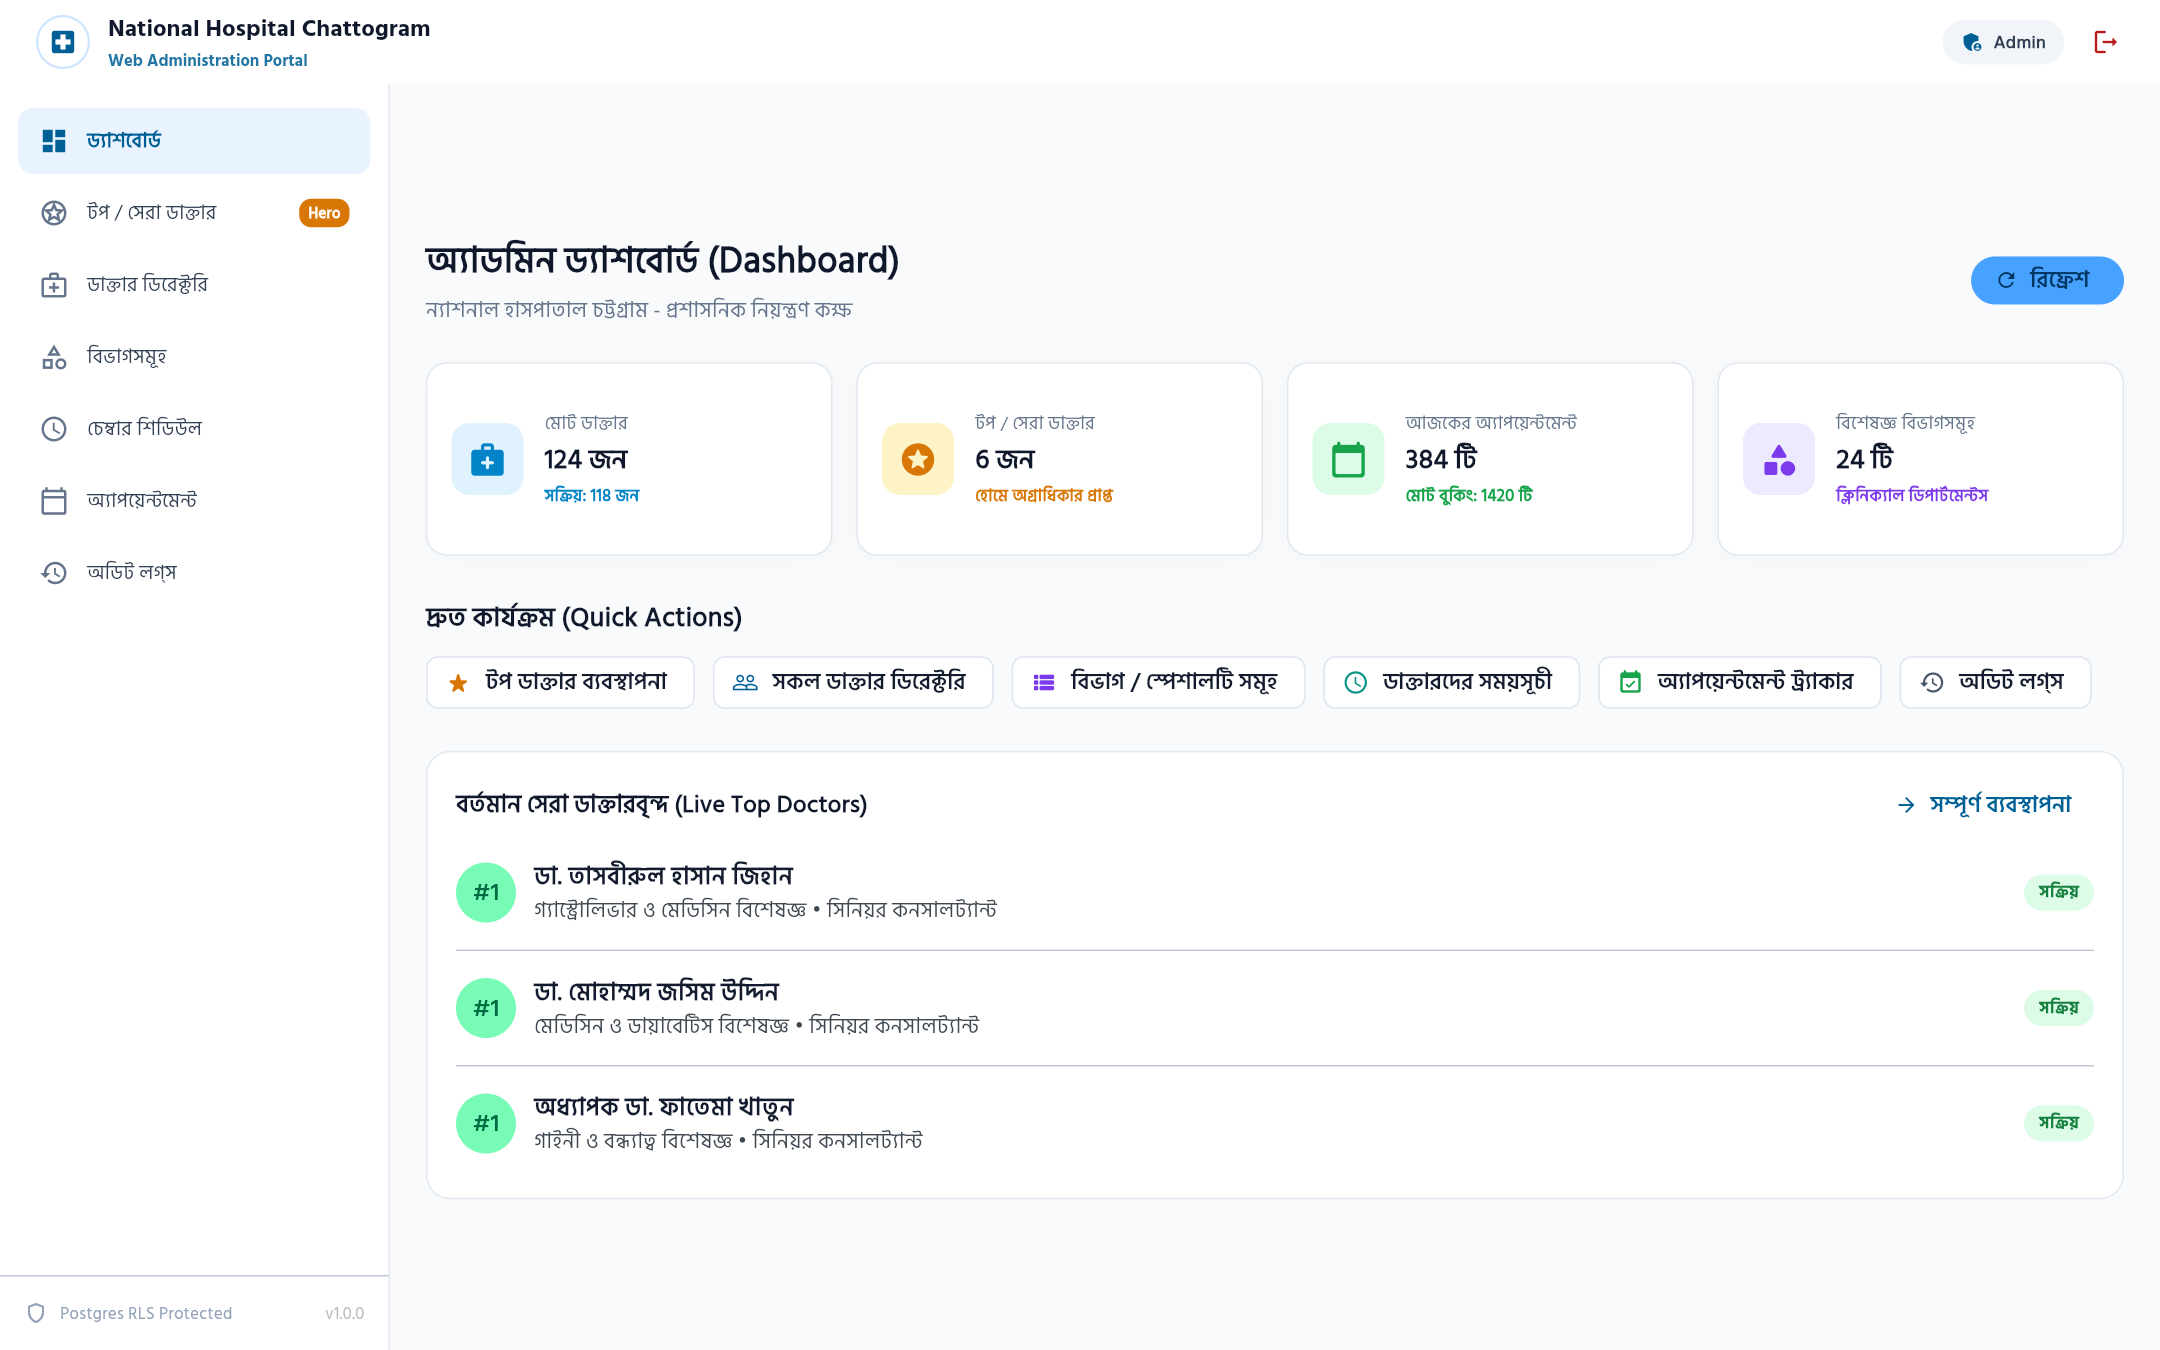
\includegraphics[width=\textwidth]{docs/screenshots/admin_dashboard.png}
        \caption{Operational Metrics and Analytics Dashboard}
        \label{fig:admin_dashboard}
    \end{subfigure}
    \\[0.3cm]
    \begin{subfigure}[b]{0.88\textwidth}
        \centering
        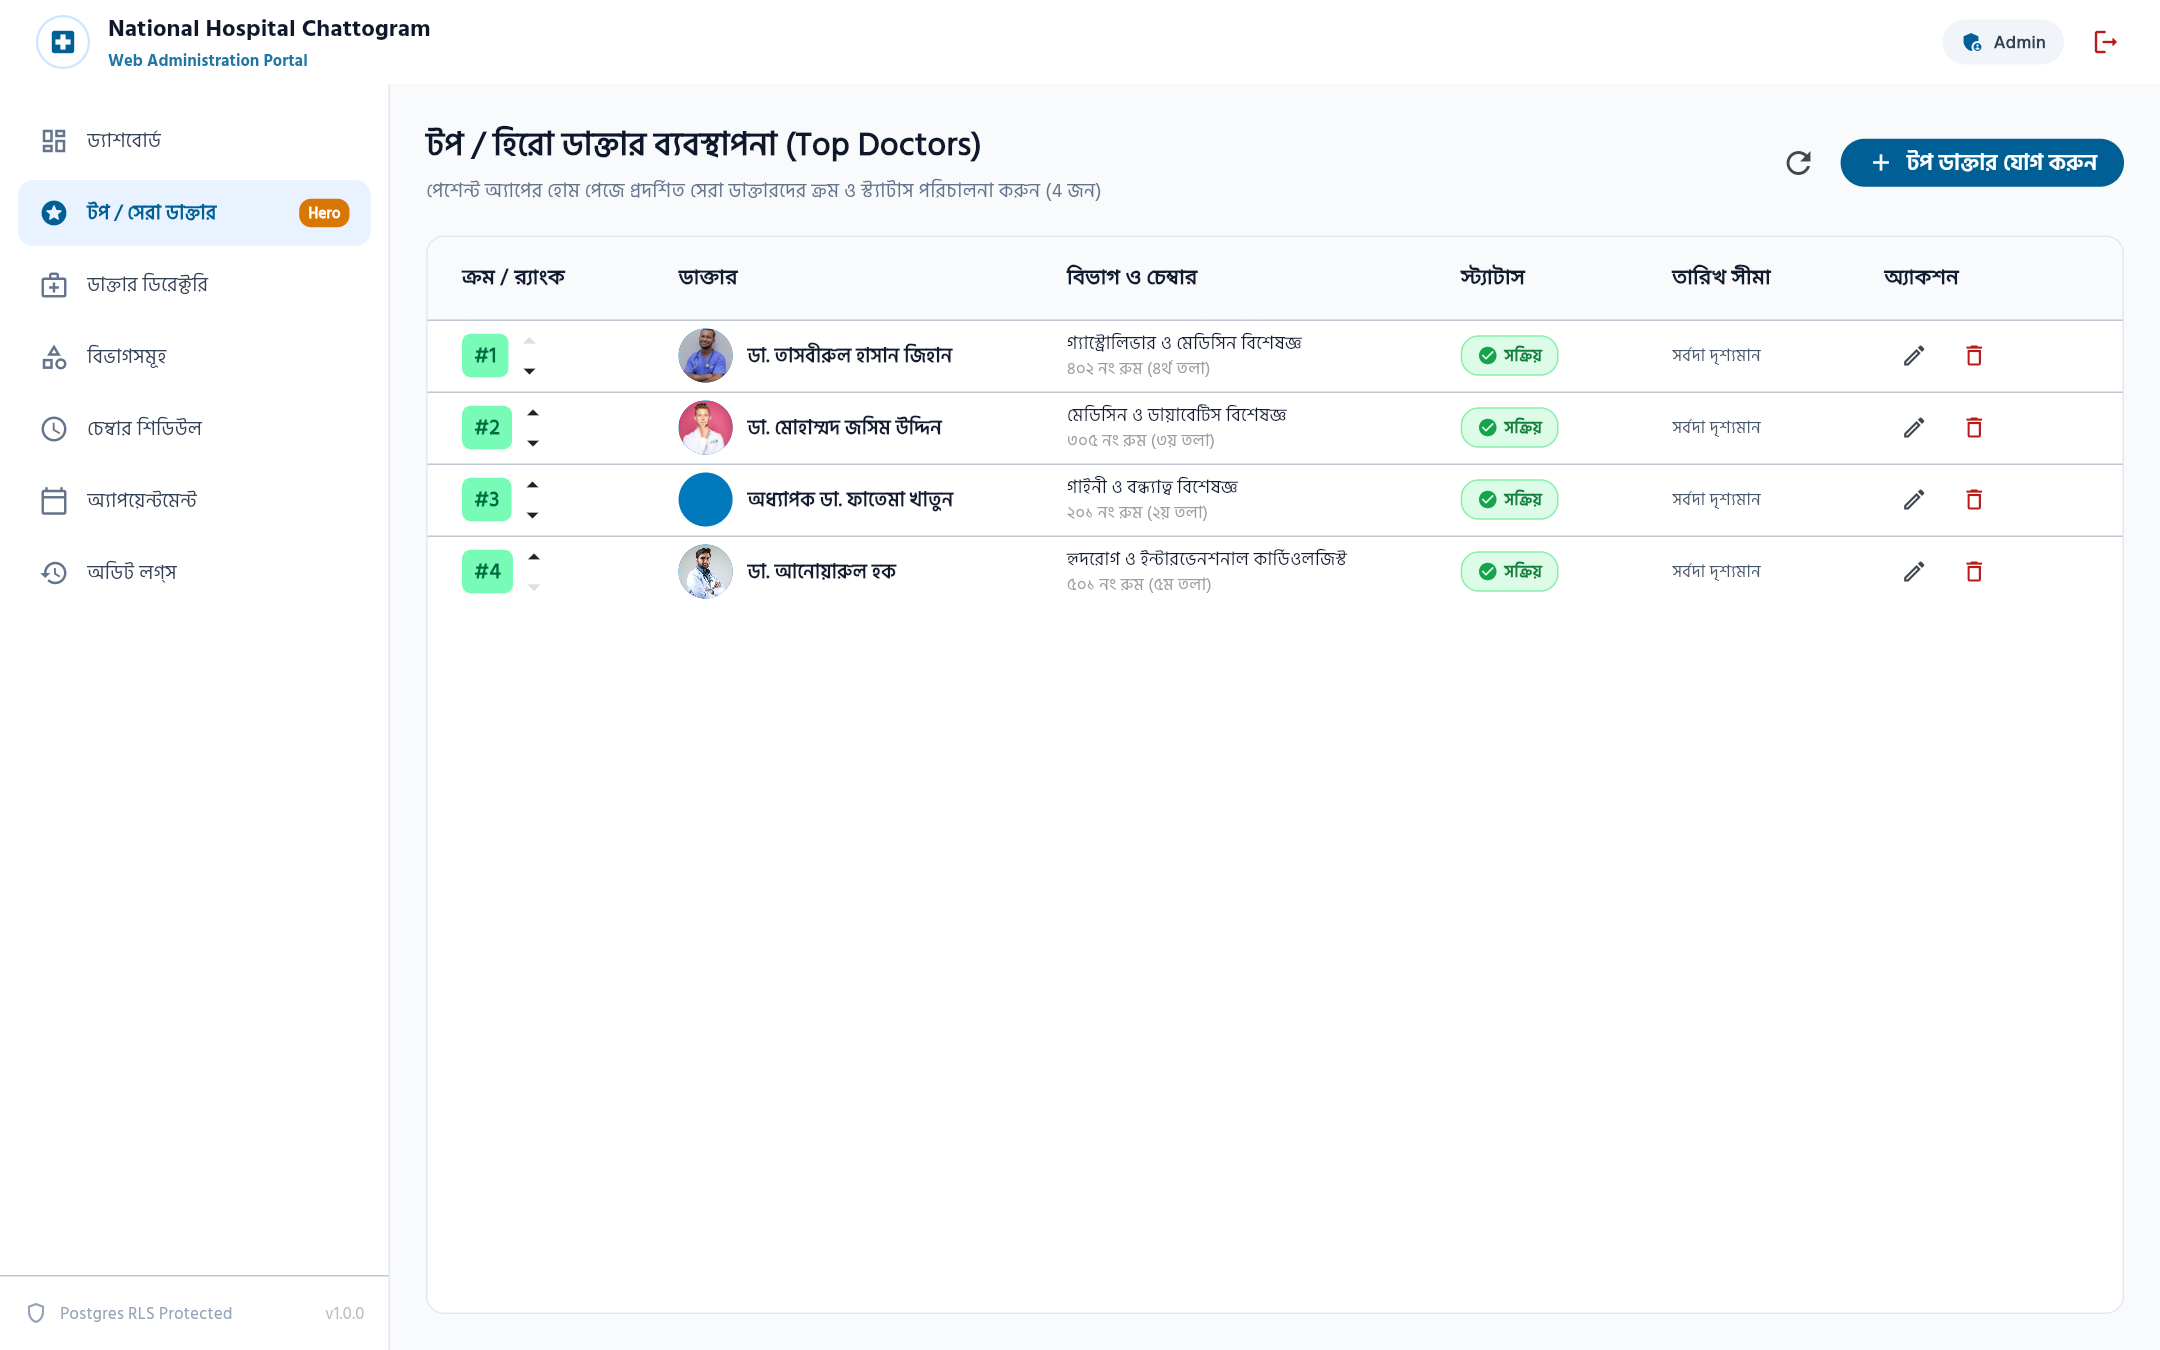
\includegraphics[width=\textwidth]{docs/screenshots/admin_top_doctors.png}
        \caption{Top Doctors Management \& Visual Reordering Console}
        \label{fig:admin_top_doctors}
    \end{subfigure}
    \caption{Web Admin Panel: Metrics Dashboard \& Top Doctors Reordering}
    \label{fig:admin_screens_1}
\end{figure}

\begin{figure}[H]
    \centering
    \begin{subfigure}[b]{0.88\textwidth}
        \centering
        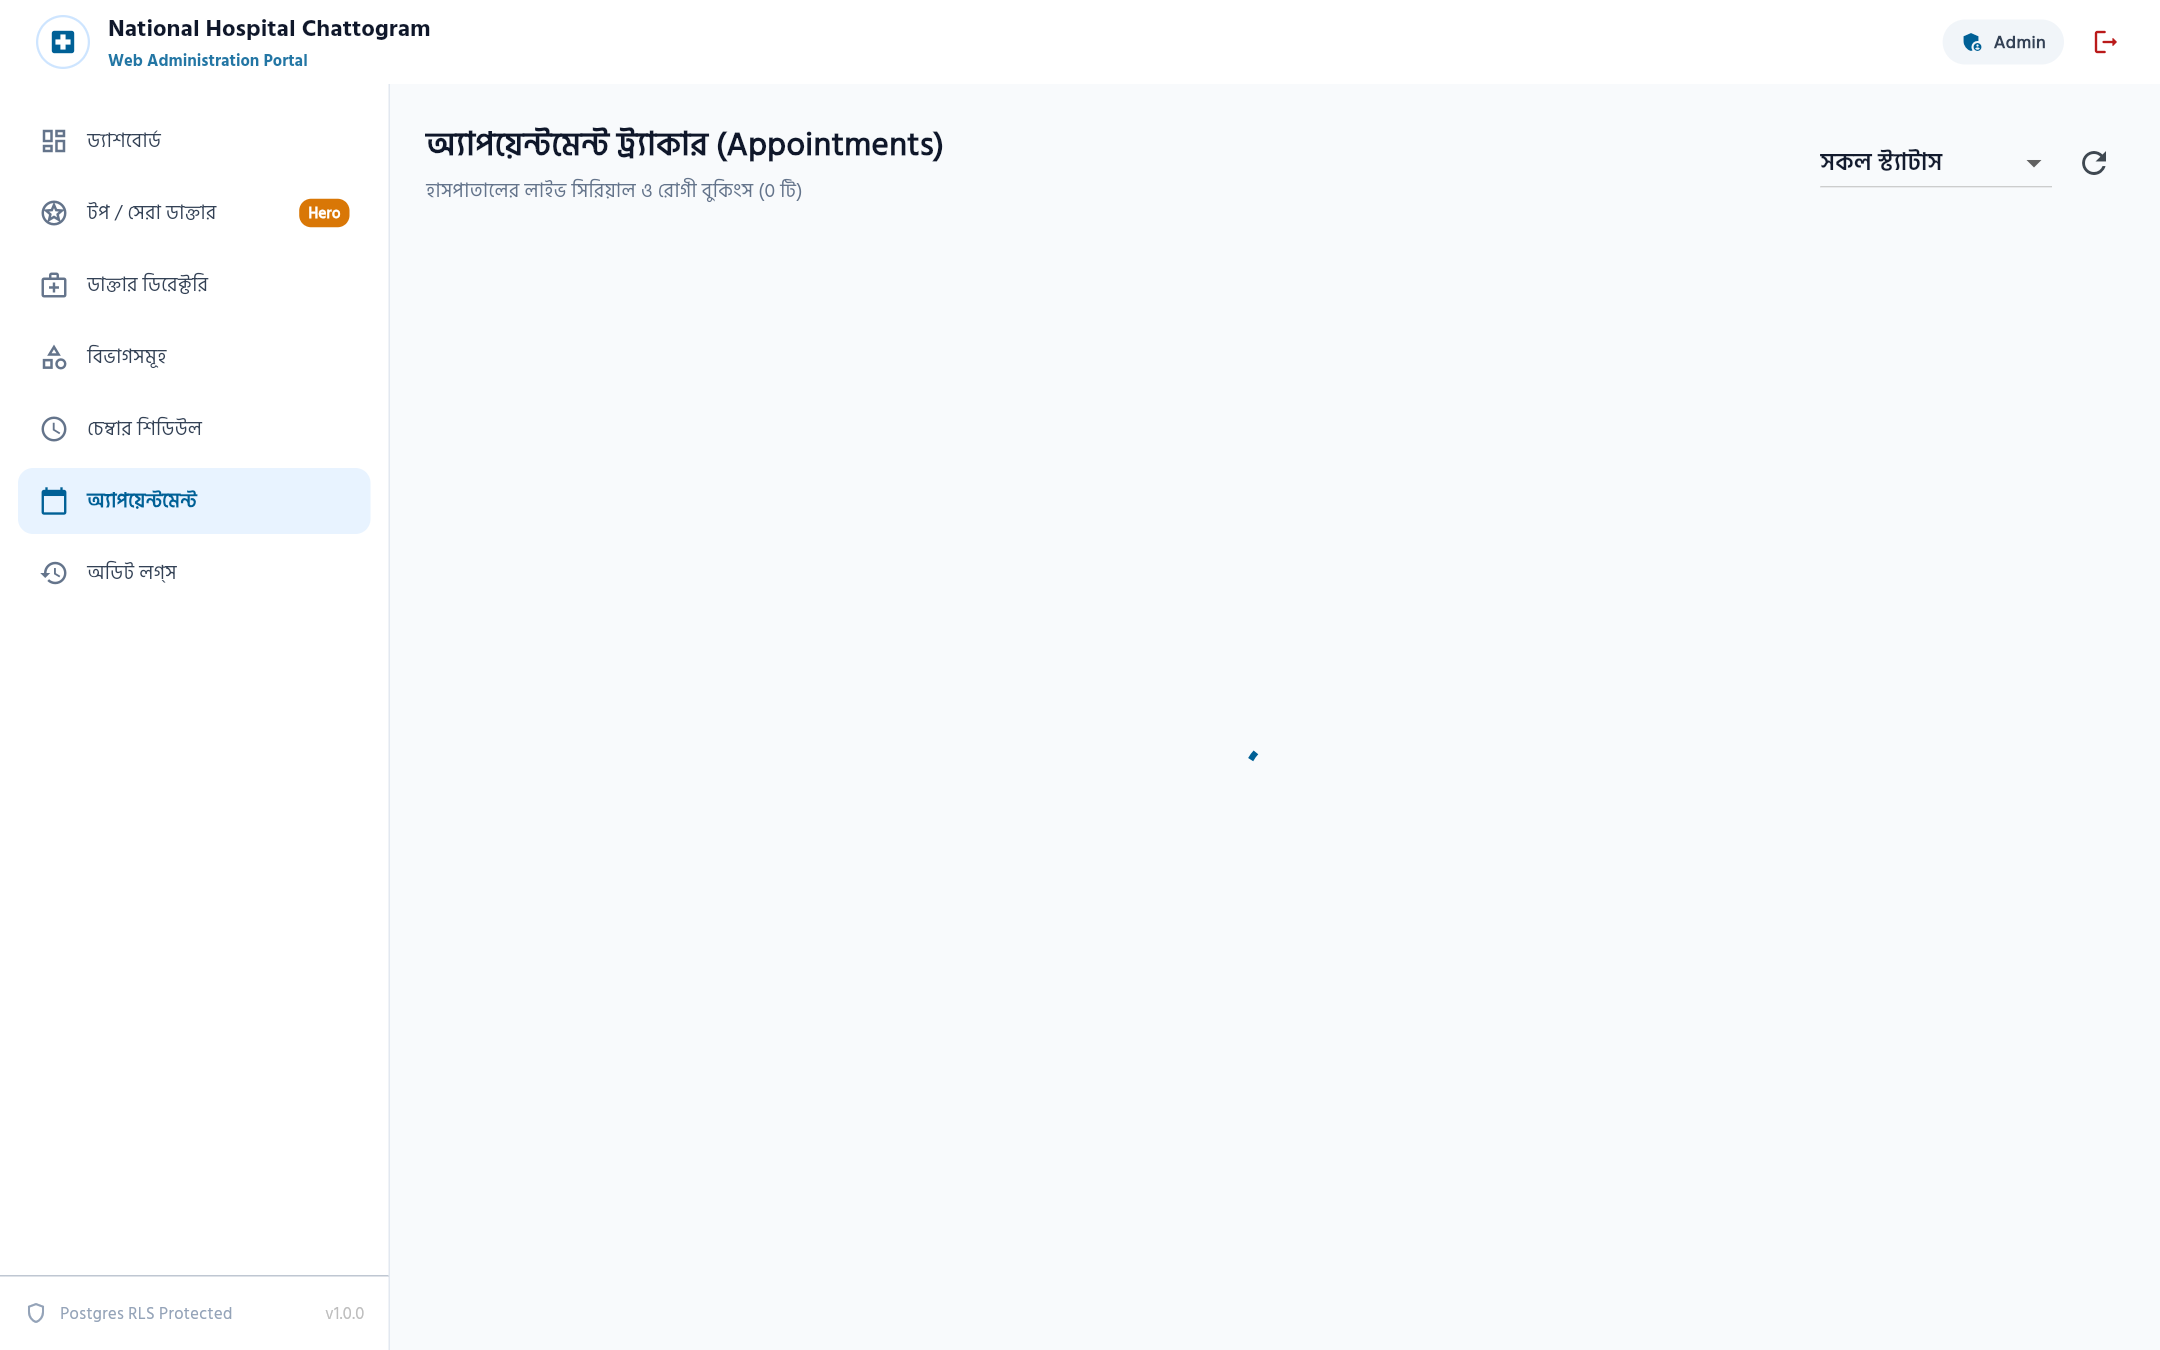
\includegraphics[width=\textwidth]{docs/screenshots/admin_appointments.png}
        \caption{Real-Time Appointment Queue Monitoring \& Status Management}
        \label{fig:admin_appointments}
    \end{subfigure}
    \\[0.3cm]
    \begin{subfigure}[b]{0.88\textwidth}
        \centering
        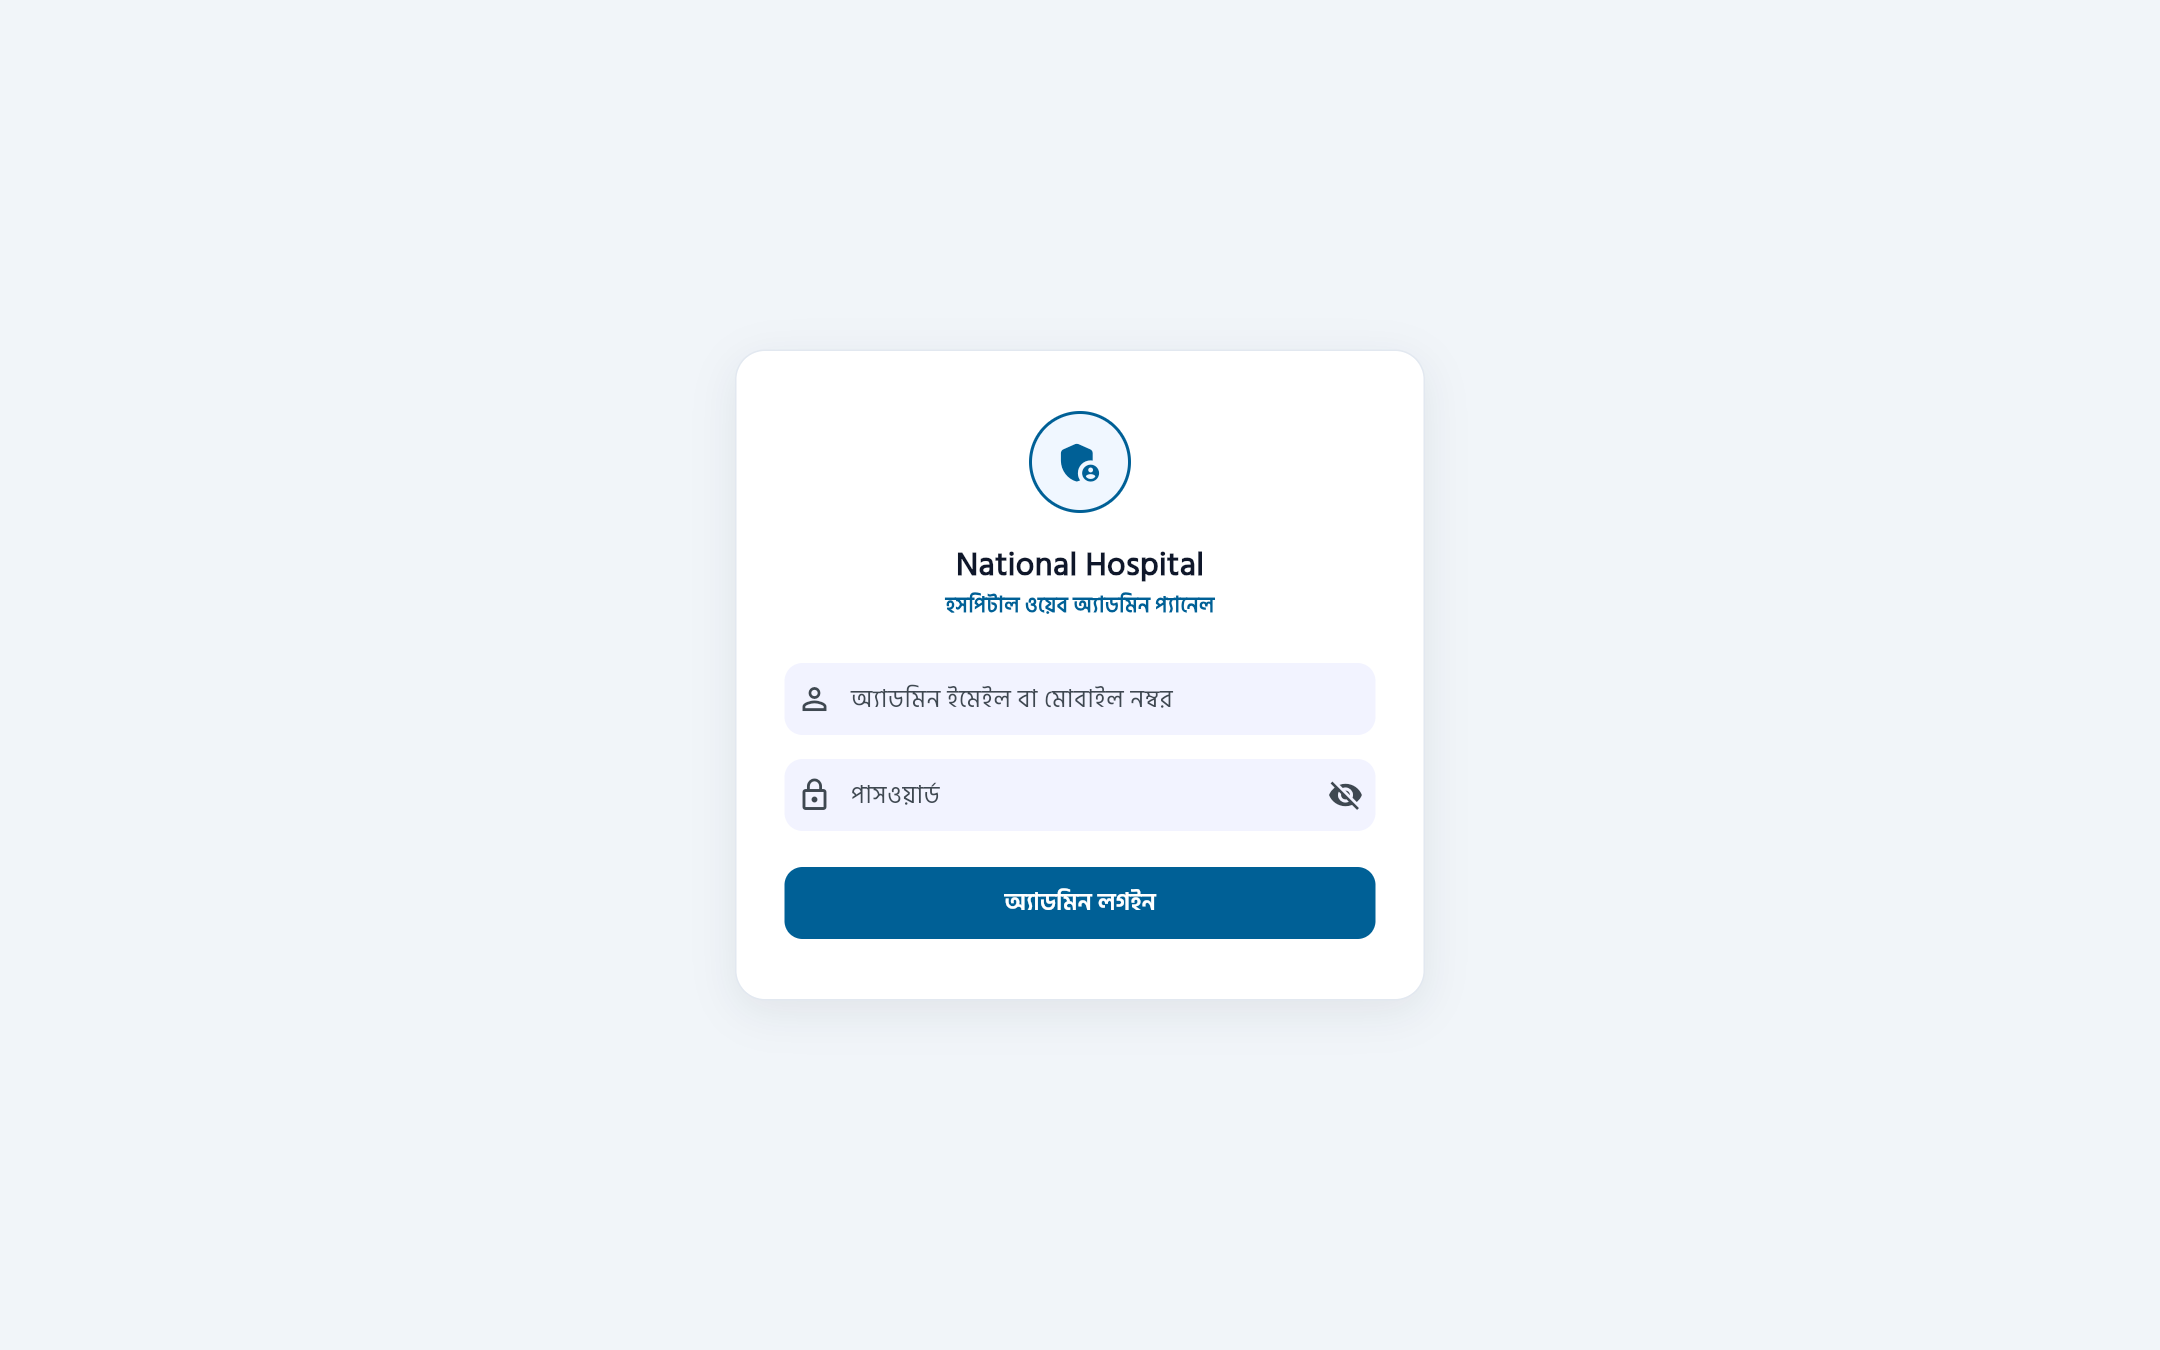
\includegraphics[width=\textwidth]{docs/screenshots/admin_login.png}
        \caption{Role-Protected Authentication Gate}
        \label{fig:admin_login}
    \end{subfigure}
    \caption{Web Admin Panel: Appointment Queue Management \& Security Gate}
    \label{fig:admin_screens_2}
\end{figure}

\clearpage
\section{Patient Mobile Application Interface}
The patient application (\texttt{/}) delivers a responsive, bilingual (Bengali/English) mobile experience for doctor discovery, live chamber visiting hours, and instant serial booking.

\begin{figure}[H]
    \centering
    \begin{subfigure}[b]{0.47\textwidth}
        \centering
        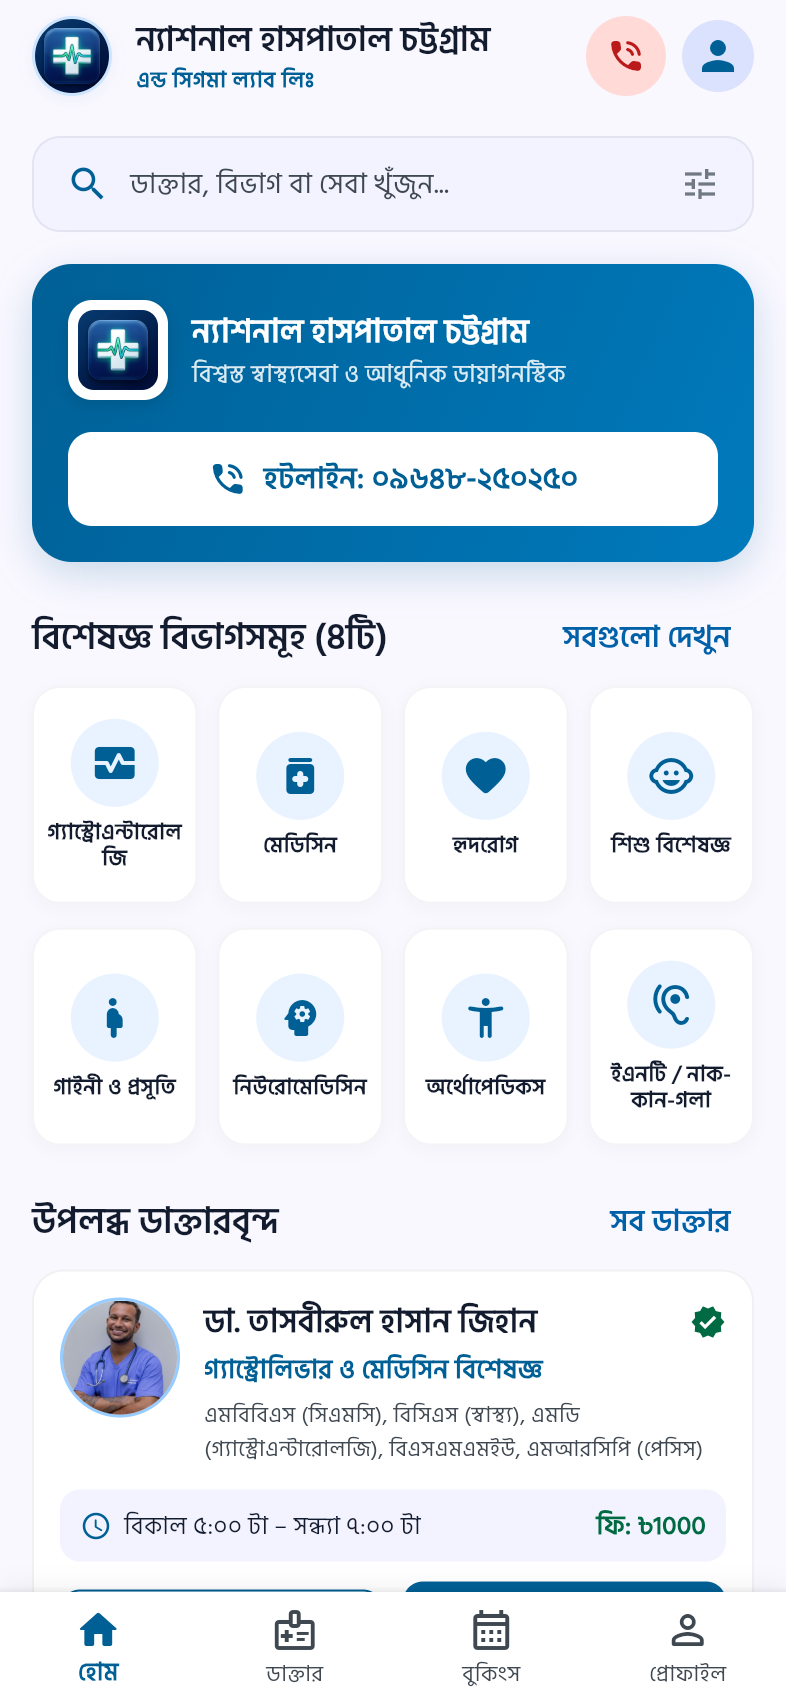
\includegraphics[width=\textwidth]{docs/screenshots/app_home_top.png}
        \caption{Patient Home Header \& Quick Services}
        \label{fig:app_home_top}
    \end{subfigure}
    \hfill
    \begin{subfigure}[b]{0.47\textwidth}
        \centering
        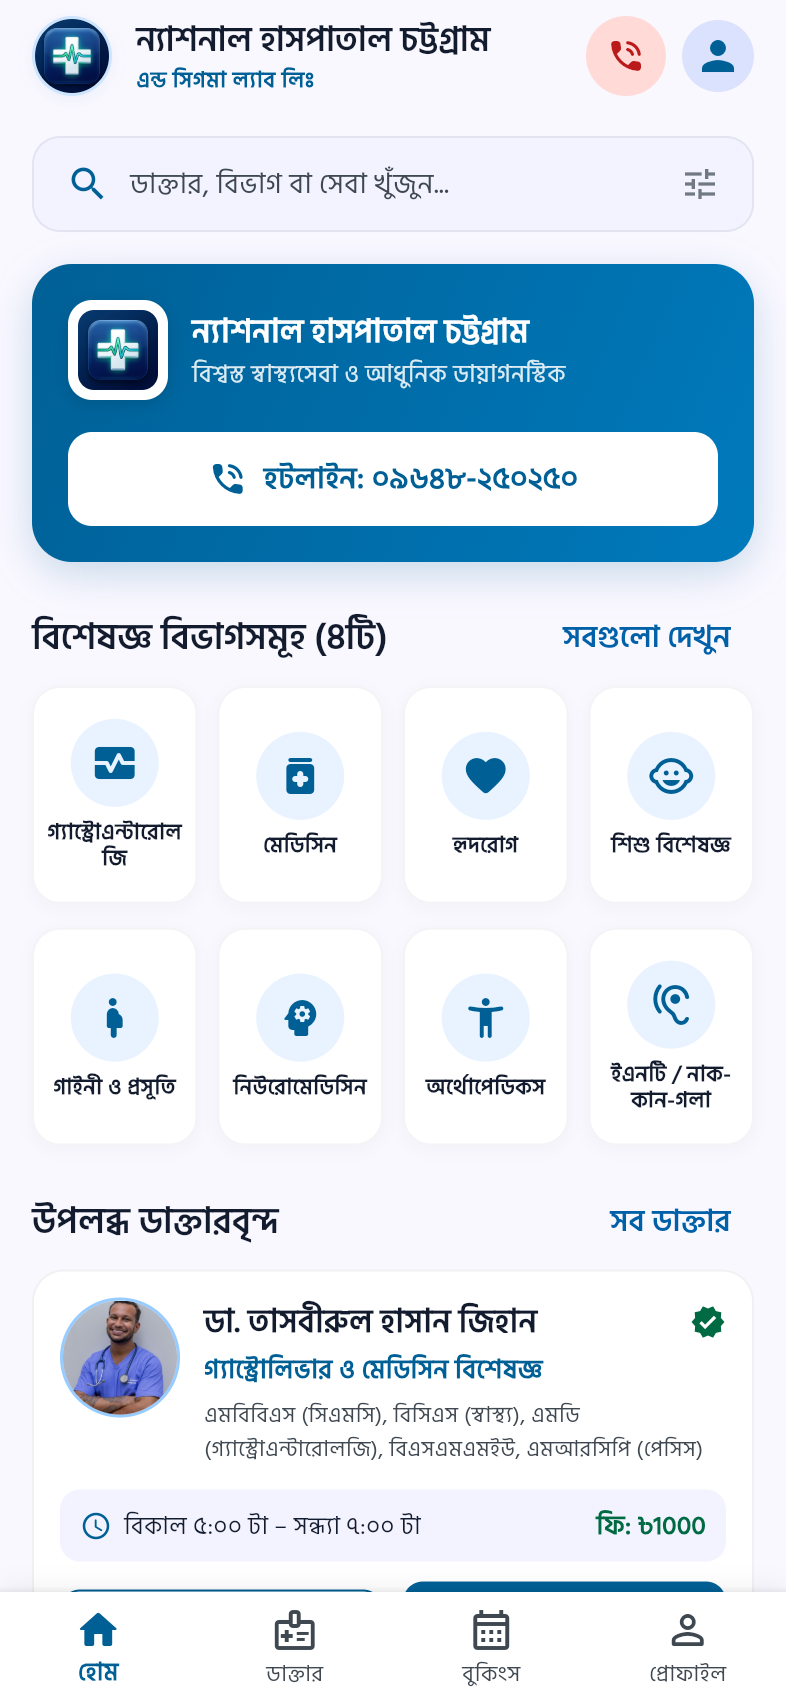
\includegraphics[width=\textwidth]{docs/screenshots/app_home_doctors.png}
        \caption{Featured Top Doctors Carousel}
        \label{fig:app_home_doctors}
    \end{subfigure}
    \caption{Patient Mobile Application: Home \& Featured Doctors}
    \label{fig:patient_app_screens_1}
\end{figure}

\begin{figure}[H]
    \centering
    \begin{subfigure}[b]{0.47\textwidth}
        \centering
        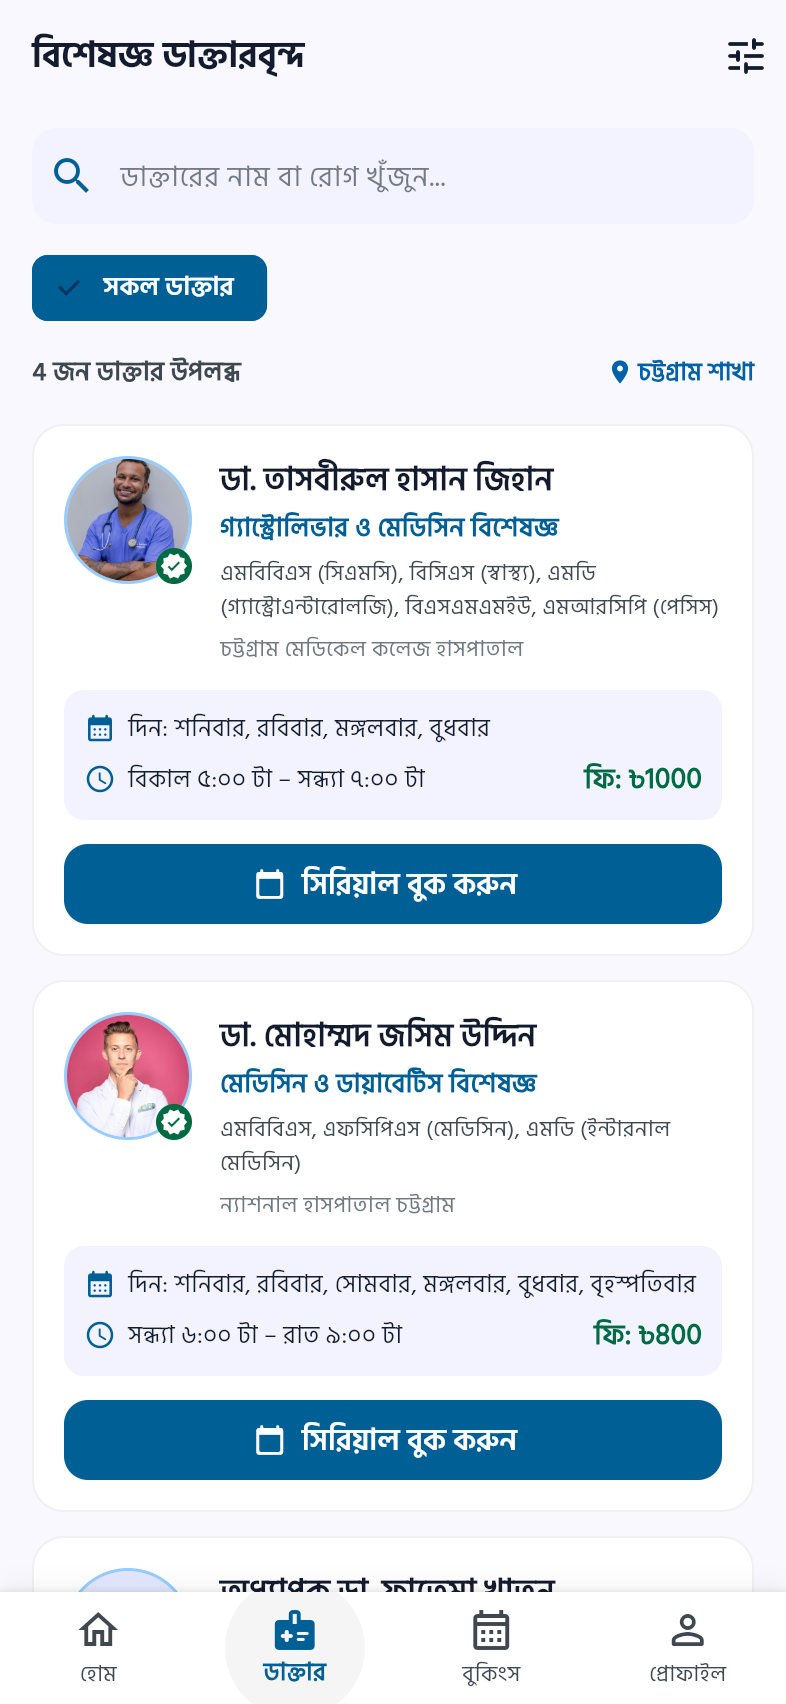
\includegraphics[width=\textwidth]{docs/screenshots/app_doctor_directory.png}
        \caption{100+ Doctor Directory with Search}
        \label{fig:app_doctor_directory}
    \end{subfigure}
    \hfill
    \begin{subfigure}[b]{0.47\textwidth}
        \centering
        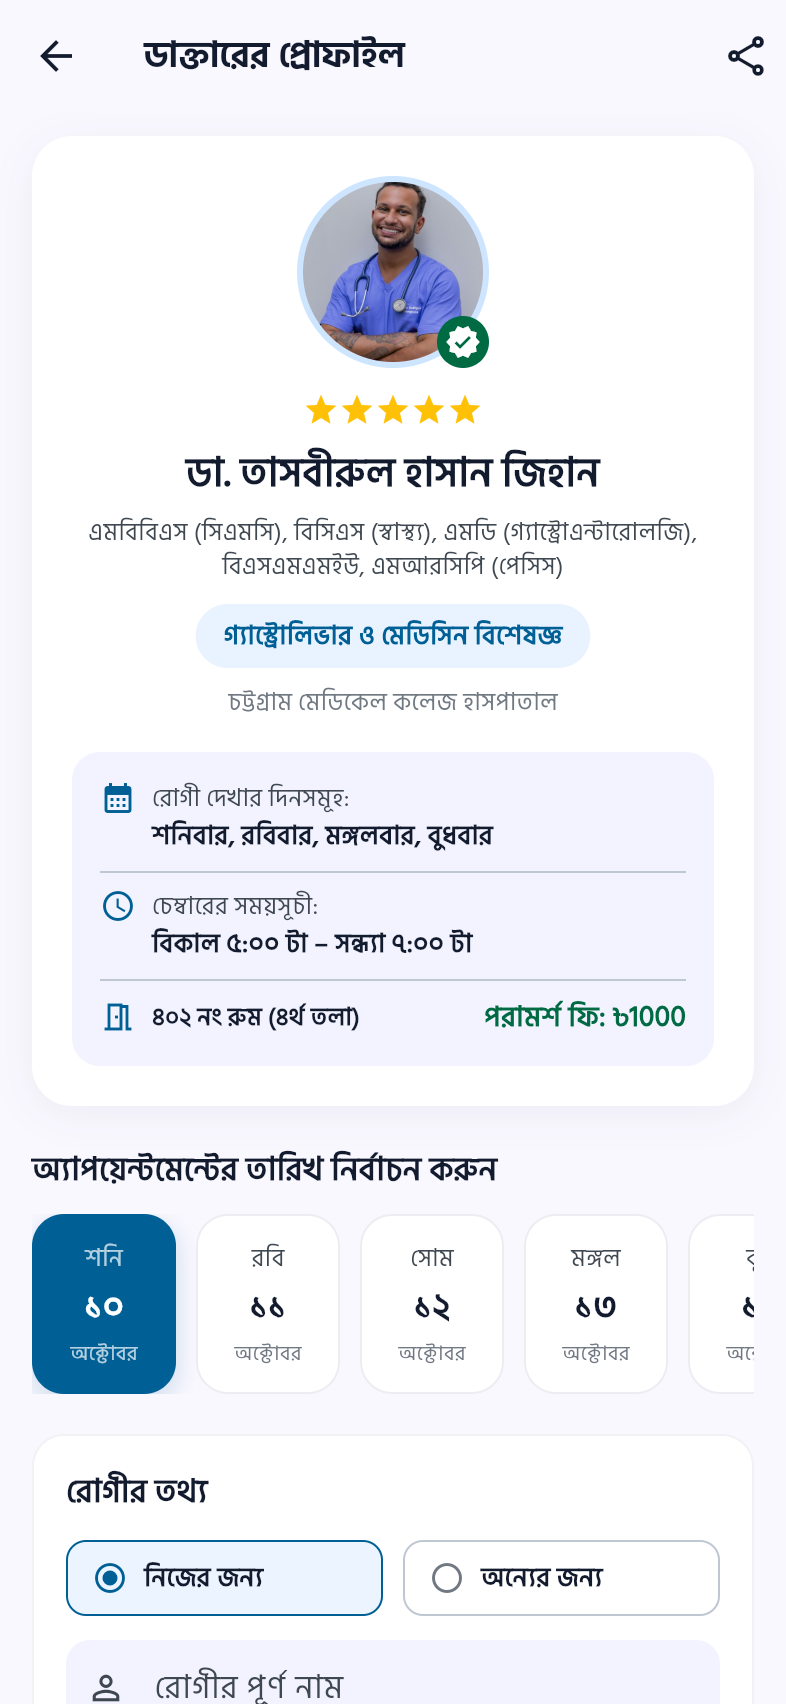
\includegraphics[width=\textwidth]{docs/screenshots/app_doctor_profile.png}
        \caption{Chamber Schedule \& Serial Booking}
        \label{fig:app_doctor_profile}
    \end{subfigure}
    \caption{Patient Mobile Application: Doctor Directory \& Chamber Booking}
    \label{fig:patient_app_screens_2}
\end{figure}

\chapter{Static Code Analysis and Automated Test Logs}
\label{app:verification}

\section{Verification Summary Matrix}
Both projects maintain 100\% clean code status and complete test suite coverage as detailed in Table~\ref{tab:test_summary}.

\begin{table}[H]
\centering
\begin{tabularx}{\textwidth}{l p{3.2cm} p{3.5cm} X}
\toprule
\textbf{Subsystem} & \textbf{Static Analysis} & \textbf{Automated Test Suite} & \textbf{Deployment Target} \\
\midrule
\textbf{Patient App} & 0 issues (\texttt{flutter analyze}) & 4/4 passing tests & Android, iOS, Web \\
\textbf{Admin Panel} & 0 issues (\texttt{flutter analyze}) & 2/2 passing tests & Flutter Web (\texttt{build/web}) \\
\bottomrule
\end{tabularx}
\caption{Subsystem Quality Assurance and Test Verification Matrix}
\label{tab:test_summary}
\end{table}

\section{Patient App Static Analysis Log}
\begin{lstlisting}[language=bash,caption={Output of flutter analyze for Patient App}]
$ cd E:/National_hospital_chattogram
$ flutter analyze
Analyzing National_hospital_chattogram...
No issues found! (ran in 25.2s)
\end{lstlisting}

\section{Admin Panel Static Analysis Log}
\begin{lstlisting}[language=bash,caption={Output of flutter analyze for Admin Panel}]
$ cd E:/National_hospital_chattogram/admin_panel
$ flutter analyze
Analyzing admin_panel...
No issues found! (ran in 6.0s)
\end{lstlisting}

\section{Patient App Automated Widget Test Execution Log}
\begin{lstlisting}[language=bash,caption={Output of flutter test for Patient App}]
$ flutter test
00:00 +0: loading E:/National_hospital_chattogram/test/widget_test.dart
00:00 +0: SplashScreen displays National Hospital and logo
00:01 +1: LoginScreen and RegisterScreen load and render properly
00:01 +2: AppRoutes generates patient routes without errors
00:01 +3: FeaturedDoctor model computes visibility and ordering correctly
00:01 +4: All tests passed!
\end{lstlisting}

\section{Admin Panel Automated Widget Test Execution Log}
\begin{lstlisting}[language=bash,caption={Output of flutter test for Standalone Web Admin Panel}]
$ cd E:/National_hospital_chattogram/admin_panel
$ flutter test
00:00 +0: loading test/widget_test.dart
00:01 +0: AdminLoginScreen renders with hospital admin branding
00:01 +1: admin_panel AppRoutes generates routes cleanly
00:01 +2: All tests passed!
\end{lstlisting}

\end{document}
